\documentclass[portuguese]{sbcreviews-2025}

% ============================================================
% PACOTES
% ============================================================

\usepackage[misc,geometry]{ifsym}
\usepackage{aas_macros}
\usepackage[bottom]{footmisc}
\usepackage{tabularray}
\usepackage{afterpage}
\usepackage{url}
\usepackage{pifont}
% ============================================================
% CONFIGURAÇÕES DO ARTIGO
% ============================================================

\setcitestyle{square}

\definecolor{engtitle}{rgb}{0.5,0.5,0.5}
\definecolor{orcidlogo}{rgb}{0.37,0.48,0.13}
\definecolor{unilogo}{rgb}{0.16,0.26,0.58}
\definecolor{maillogo}{rgb}{0.58,0.16,0.26}
\definecolor{darkblue}{rgb}{0.0,0.0,0.0}

\hypersetup{
    colorlinks,
    breaklinks,
    linkcolor=darkblue,
    urlcolor=darkblue,
    anchorcolor=darkblue,
    citecolor=darkblue
}

% ============================================================
% INFORMAÇÕES DA PUBLICAÇÃO
% ============================================================

\jid{ROCS}
\jtitle{Trabalho Prático de Projeto de Software, 2026}
\issn{}
\doi{}

\copyrightstatement{
    This work is licensed under a Creative Commons
    Attribution 4.0 International License
}

\jyear{2026}
\category{Trabalho Prático}

% ============================================================
% TÍTULO
% ============================================================

\title[DevMatch]{
    DevMatch: Especificação e Modelagem de uma Plataforma de
    Marketplace para Contratação de Profissionais de TI Freelancers
}

\engtitle{
    \textcolor{engtitle}{
        DevMatch: Specification and Modeling of a Marketplace
        Platform for Hiring Freelance IT Professionals
    }
}

% ============================================================
% AUTORES
% Substituir os ORCIDs quando os integrantes possuírem
% ============================================================

\author[Andrade et al. 2026]{

\affil{
    \textbf{Antônio Henrique Rabelo Andrade}
    
    [PUC Minas |
    \href{mailto:ahrandrade@sga.pucminas.br}
    {\textit{ahrandrade@sga.pucminas.br}}]
}

\affil{
    \textbf{João Pedro Bomfim Victor}
    
    [PUC Minas |
    \href{mailto:joao.bomfim@sga.pucminas.br}
    {\textit{joao.bomfim@sga.pucminas.br}}]
}

\affil{
    \textbf{Júlia de Souza Ventura}
    
    [PUC Minas |
    \href{mailto:jsventura@sga.pucminas.br}
    {\textit{jsventura@sga.pucminas.br}}]
}

\affil{
    \textbf{Pedro Henrique Germano de Melo Santos}
    
    [PUC Minas |
    \href{mailto:pedro.germano@sga.pucminas.br}
    {\textit{pedro.germano@sga.pucminas.br}}]
}

\affil{
    \textbf{Yuri Cardoso Viana}
    
    [PUC Minas |
    \href{mailto:ycviana@sga.pucminas.br}
    {\textit{ycviana@sga.pucminas.br}}]
}

}

% ============================================================
% INÍCIO DO DOCUMENTO
% ============================================================

\begin{document}

\begin{frontmatter}

\maketitle

\begin{mail}
Curso de Engenharia de Software,
Pontifícia Universidade Católica de Minas Gerais (PUC Minas),
Belo Horizonte, MG, Brasil.
\end{mail}

% ============================================================
% RESUMO
% ============================================================

\begin{abstract-pt}
Este artigo especifica o DevMatch, marketplace de contratação de profissionais de TI freelancers. A proposta integra publicação de projetos, recomendação, contratos por marcos, custódia de pagamentos e mediação de disputas. Com base no enunciado, foram descritos quatro atores, casos de uso e histórias de usuário com critérios de aceitação. O resultado é uma especificação inicial do fluxo de contratação, que orienta a modelagem de projeto e de dados. Implementação e validação com usuários são etapas futuras.
\end{abstract-pt}

% ============================================================
% ABSTRACT
% ============================================================

\begin{abstract-en}
This article specifies DevMatch, a marketplace for hiring freelance IT professionals. The proposal combines project posting, recommendations, milestone contracts, escrow payments, and dispute mediation. Based on the system brief, four actors, use cases, and user stories with acceptance criteria were described. The result is an initial specification of the hiring workflow that guides the design and data models. Implementation and validation with users remain future work.
\end{abstract-en}

\begin{pchaves}
Marketplace de Freelancers, Engenharia de Software,
Modelagem de Sistemas, UML
\end{pchaves}

\begin{keywords}
Freelancer Marketplace, Software Engineering,
System Modeling, UML
\end{keywords}



\end{frontmatter}

% ============================================================
% 1 INTRODUÇÃO
% ============================================================

\section{Introdução}
\label{sec:intro}

A expansão das plataformas digitais modificou a forma como empresas
e profissionais estabelecem relações de trabalho. No setor de
tecnologia da informação, essas plataformas possibilitam que
organizações e pessoas contratem profissionais independentes para
desenvolver sistemas, aplicativos, páginas Web, integrações,
automações e outros produtos de software. Ao mesmo tempo,
profissionais freelancers podem encontrar oportunidades sem as
limitações geográficas de processos tradicionais de contratação.
A existência de mercados de trabalho mediados por plataformas
reforça a relevância de estudar esse modelo de contratação \citep{kassi2018}.

Apesar de suas vantagens, a contratação remota de serviços de
desenvolvimento de software envolve riscos para clientes e
freelancers. Os clientes podem encontrar dificuldades para avaliar
as competências técnicas dos candidatos, verificar seus históricos
profissionais e acompanhar a execução do trabalho contratado. Por
outro lado, freelancers estão sujeitos a alterações de escopo,
requisitos pouco claros, atrasos na aprovação das entregas e falta
de pagamento. Em ambientes digitais, mecanismos de reputação,
avaliação e rastreabilidade são importantes para reduzir incertezas
e apoiar a construção de confiança entre participantes que não
possuem uma relação anterior \citep{josang2007}.

Nesse contexto, propõe-se o DevMatch, uma plataforma de marketplace
destinada a conectar profissionais de tecnologia freelancers a
empresas ou pessoas físicas que necessitam contratar serviços de
desenvolvimento de software. O sistema permite que clientes publiquem
projetos contendo escopo, prazo, orçamento estimado e tecnologias
exigidas. Os freelancers, por sua vez, podem cadastrar suas
competências, portfólio, certificações, disponibilidade e valor de
trabalho, além de localizar projetos e enviar propostas comerciais.

A proposta do DevMatch integra mecanismos voltados à
confiança e à segurança da contratação. Entre eles estão a
recomendação inteligente de projetos e profissionais, a verificação
de competências por meio de testes técnicos, a avaliação
bidirecional, o acompanhamento por marcos de entrega e o pagamento
em custódia. Nesse modelo, o valor de cada marco permanece em custódia
até a aprovação da entrega ou a resolução de uma disputa, segundo
as regras contratuais. O sistema também permite a abertura
de disputas, a mediação por administradores e a manutenção de
registros auditáveis das alterações contratuais e transações
financeiras.

O objetivo geral deste trabalho é especificar e modelar o sistema
DevMatch, aplicando conceitos de engenharia de requisitos, modelagem
UML, arquitetura de software e modelagem de dados. Como objetivos
específicos, busca-se identificar os atores e suas
responsabilidades; levantar requisitos funcionais e não funcionais;
representar as interações por meio de casos de uso e histórias de
usuário; definir a arquitetura do sistema; elaborar diagramas
estruturais e comportamentais; e desenvolver os modelos conceitual,
lógico e físico do banco de dados. O processo de levantamento e
documentação dos requisitos segue princípios de definição, análise
e especificação de necessidades estabelecidos pela engenharia de
requisitos \citep{iso29148}.

Este artigo está organizado da seguinte maneira: após esta introdução,
são apresentados os trabalhos relacionados e as características que
diferenciam o DevMatch de soluções semelhantes. Em seguida, a seção
de modelagem de requisitos descreve os atores, os casos de uso, as
histórias de usuário, os diagramas de sequência do sistema e os
contratos de operação. Posteriormente, são apresentadas a arquitetura
e as modelagens de projeto e de dados. Por fim, são discutidos os
resultados da modelagem e apresentadas as considerações finais do
trabalho.

% ============================================================
% 2 TRABALHOS RELACIONADOS
% Será preenchido pelo integrante responsável
% ============================================================

\section{Trabalhos Relacionados}
\label{sec:trabalhos-relacionados}

% Inserir aqui a análise dos sistemas semelhantes ao DevMatch.

% ============================================================
% 3 MODELAGEM DE REQUISITOS
% ============================================================

\section{Modelagem de Requisitos}
\label{sec:requisitos}

A modelagem de requisitos do DevMatch tem como finalidade definir as
responsabilidades dos participantes e delimitar as funcionalidades
pertencentes ao escopo da plataforma. Os requisitos foram obtidos a
partir da análise do contexto do sistema, considerando o ciclo
completo de contratação: publicação do projeto, busca e recomendação
de profissionais, envio de propostas, formalização do contrato,
acompanhamento das entregas, pagamento, disputa e avaliação.

Os comportamentos identificados foram representados por meio de casos
de uso, seguindo a notação da Unified Modeling Language (UML)
\citep{omguml}. As necessidades dos participantes também foram
documentadas como histórias de usuário, permitindo relacionar cada
funcionalidade ao benefício esperado por seu respectivo ator.

% ============================================================
% 3.1 DESCRIÇÃO DOS ATORES
% ============================================================

\subsection{Descrição dos Atores}
\label{subsec:atores}

Um ator representa um papel externo que interage com o sistema para
atingir determinado objetivo. No DevMatch foram identificados quatro
atores principais: freelancer, cliente, administrador do sistema e
analista financeiro ou de suporte. A Tabela~\ref{tab:atores}
apresenta os objetivos e as principais interações de cada um deles.

\begin{table*}[!ht]
\caption{Atores e suas interações com o DevMatch.}
\label{tab:atores}
\centering

\begin{tblr}{
    width=\textwidth,
    colspec={
        Q[l,wd=0.16\textwidth]
        Q[l,wd=0.25\textwidth]
        X[l]
    },
    row{1}={
        font=\bfseries,
        bg=gray!15
    },
    cells={
        valign=m
    },
    hlines,
    vlines
}

Ator & Objetivo & Interações com o sistema \\

Freelancer &
Encontrar oportunidades e prestar serviços de tecnologia de forma
segura. &
Cria e atualiza seu perfil profissional; informa competências,
portfólio, certificações, disponibilidade e valor; realiza testes
técnicos; pesquisa projetos; recebe recomendações; envia e negocia
propostas; acompanha contratos e marcos; registra entregas; recebe
pagamentos; abre disputas; e avalia clientes. \\

Cliente &
Contratar profissionais adequados e acompanhar a execução dos
projetos. &
Cadastra projetos com escopo, prazo, orçamento e tecnologias; recebe
recomendações de freelancers; analisa e negocia propostas; contrata
profissionais; deposita valores em custódia; acompanha o progresso;
aprova ou rejeita entregas; libera pagamentos; abre disputas; e
avalia freelancers. \\

Administrador &
Garantir a segurança, a integridade e o funcionamento adequado da
plataforma. &
Gerencia usuários, perfis e permissões; acompanha verificações de
identidade; bloqueia contas quando necessário; consulta logs e
registros de auditoria; analisa comportamentos suspeitos; e realiza
a mediação de disputas entre clientes e freelancers. \\

Analista financeiro/suporte &
Administrar operações financeiras e atender solicitações relacionadas
ao uso da plataforma. &
Acompanha depósitos em custódia; valida repasses e reembolsos;
consulta transações; emite relatórios financeiros e de comissões;
investiga falhas de pagamento; e atende chamados de clientes e
freelancers. \\

\end{tblr}
\end{table*}

O freelancer e o cliente são os atores diretamente envolvidos na
contratação e execução de um projeto. O administrador e o analista
financeiro ou de suporte são atores internos da organização
responsável pelo DevMatch. Embora possuam acesso a informações
operacionais, suas permissões devem ser limitadas conforme suas
responsabilidades, respeitando os requisitos de privacidade,
segurança e rastreabilidade.

Serviços externos, como processadores de pagamento, mecanismos de
autenticação e serviços de notificação, podem participar da execução
técnica das funcionalidades. Entretanto, eles são considerados
sistemas de apoio e não substituem os quatro atores de negócio
identificados.

% ============================================================
% 3.2 CASOS DE USO
% ============================================================

\subsection{Modelo de Casos de Uso}
\label{subsec:casos-de-uso}

O modelo de casos de uso apresenta uma visão geral das funcionalidades
oferecidas pelo DevMatch e das relações entre essas funcionalidades
e seus atores principais. O diagrama da
Figura~\ref{fig:casos-de-uso} apresenta esses objetivos de
negócio; o catálogo complementa as interações compartilhadas.

\begin{figure*}[!ht]
\centering
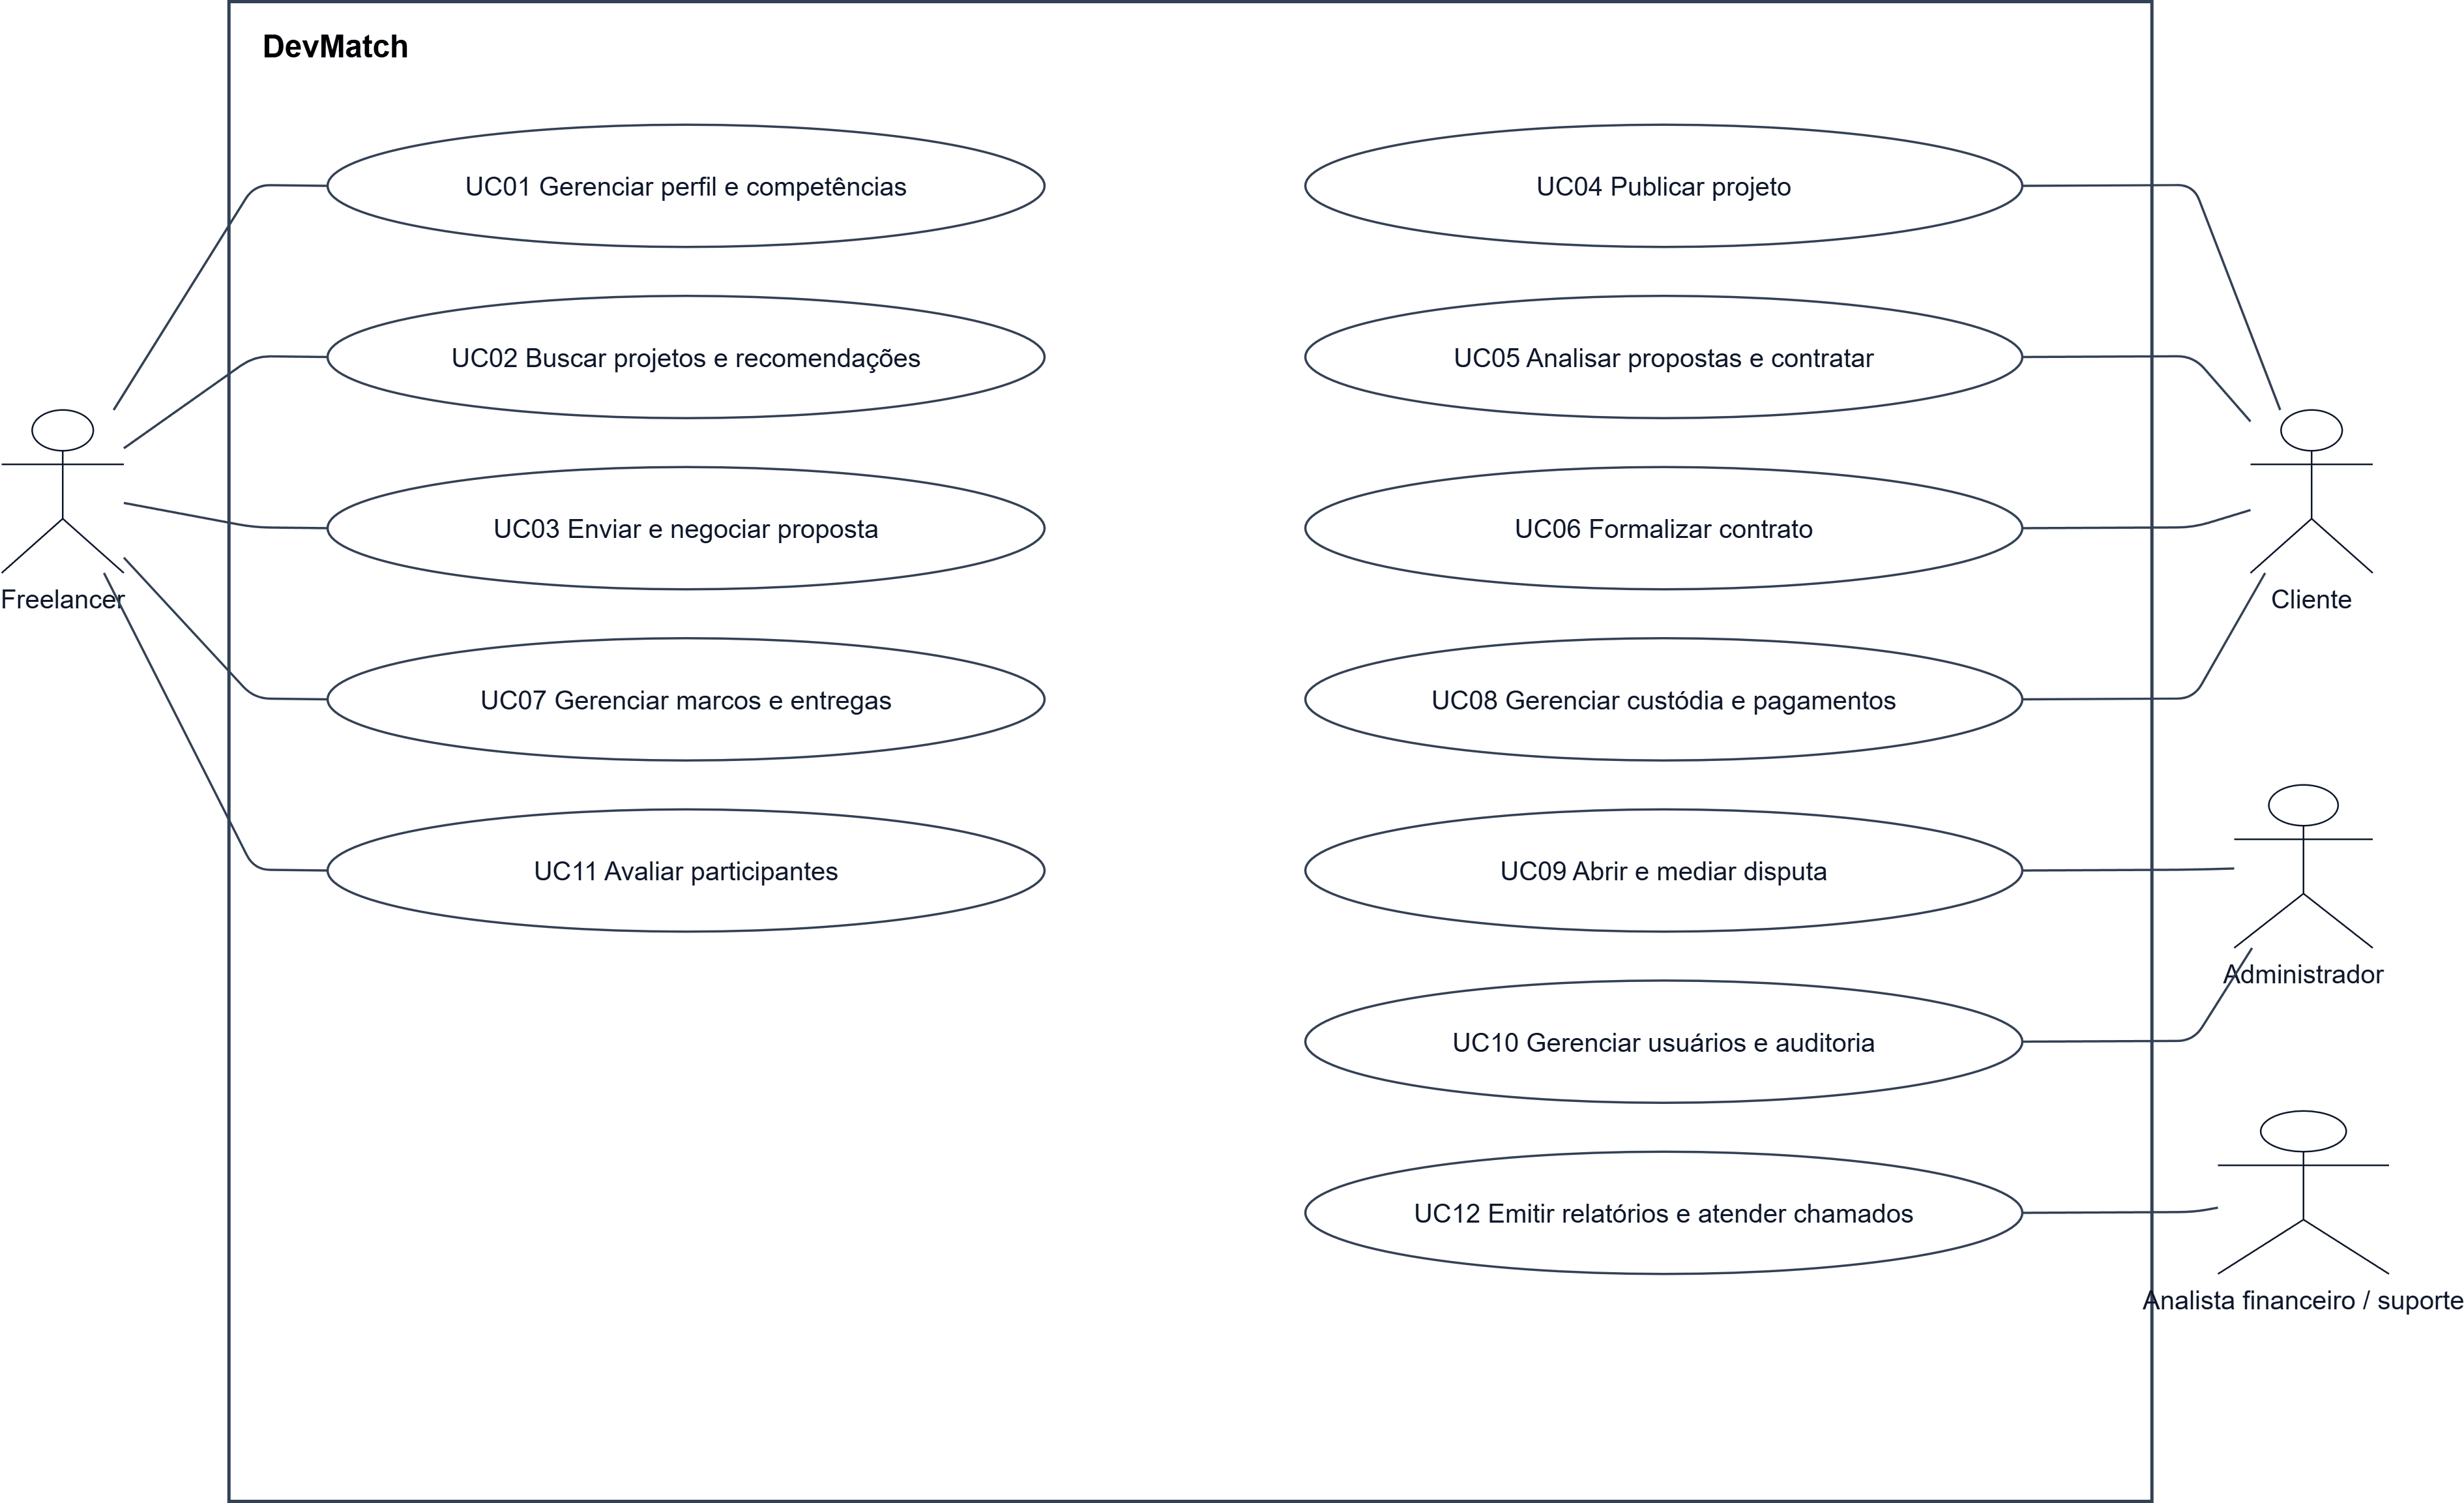
\includegraphics[width=0.8\textwidth]{casos_de_uso.png}
\caption{Visão geral dos casos de uso do DevMatch. As associações destacam o ator principal; os demais participantes são descritos no catálogo.}
\label{fig:casos-de-uso}
\end{figure*}

O caso de uso de gerenciamento de perfil inclui o registro de
competências, portfólio, certificações, disponibilidade e valor de
trabalho do freelancer. A comprovação de competências ocorre por meio de testes
técnicos associados a tecnologias específicas, com resultado
registrado no perfil.
O mecanismo de recomendação considera stack, disponibilidade,
histórico de avaliações e faixa de preço para sugerir projetos
a freelancers e profissionais a clientes. As sugestões auxiliam a
escolha, sem realizar contratações automaticamente.

Após a publicação de um projeto, os freelancers podem enviar propostas
contendo valor, prazo e observações. Quando uma proposta é aceita,
cliente e freelancer formalizam um contrato e definem os marcos de
entrega. O cliente realiza o depósito do valor acordado no sistema de
custódia, e o pagamento é liberado de acordo com a aprovação das
entregas. Caso exista desacordo, uma disputa pode ser aberta e
encaminhada para mediação.

A Tabela~\ref{tab:catalogo-casos-uso} apresenta o catálogo dos
principais casos de uso identificados.

\begin{table*}[!ht]
\caption{Catálogo dos principais casos de uso do DevMatch.}
\label{tab:catalogo-casos-uso}
\centering

\begin{tblr}{
    width=\textwidth,
    colspec={
        Q[c,wd=0.07\textwidth]
        Q[l,wd=0.23\textwidth]
        Q[l,wd=0.20\textwidth]
        X[l]
    },
    row{1}={
        font=\bfseries,
        bg=gray!15
    },
    cells={
        valign=m,
        font=\scriptsize
    },
    hlines,
    vlines
}

Código & Caso de uso & Ator principal & Objetivo \\

UC01 &
Gerenciar perfil e competências &
Freelancer &
Cadastrar e manter informações profissionais, portfólio,
certificações, disponibilidade, valor e resultados de testes
técnicos. \\

UC02 &
Buscar e consultar recomendações &
Freelancer e cliente &
Localizar projetos por filtros e visualizar oportunidades sugeridas
ao freelancer ou profissionais sugeridos ao cliente. \\

UC03 &
Enviar e negociar proposta &
Freelancer &
Apresentar ao cliente uma proposta contendo valor, prazo e condições,
permitindo ajustes durante a negociação. \\

UC04 &
Publicar e gerenciar projeto &
Cliente &
Cadastrar um projeto com escopo, prazo, orçamento, tecnologias e
demais informações necessárias à contratação. \\

UC05 &
Analisar propostas e contratar freelancer &
Cliente &
Comparar propostas e perfis para selecionar o profissional
responsável pela execução do projeto. \\

UC06 &
Formalizar e acompanhar contrato &
Cliente e freelancer &
Registrar o acordo entre as partes, incluindo escopo, valor, prazo,
responsabilidades e situação do contrato. \\

UC07 &
Gerenciar marcos e entregas &
Cliente e freelancer &
Definir marcos, registrar entregas, solicitar ajustes e acompanhar
o progresso do projeto. \\

UC08 &
Gerenciar custódia, pagamentos e repasses &
Cliente e analista financeiro &
Registrar depósitos, manter valores em custódia, liberar pagamentos
após aprovação ou mediação, executar repasses e tratar reembolsos. \\

UC09 &
Abrir e mediar disputa &
Cliente, freelancer e administrador &
Registrar um desacordo, anexar evidências, acompanhar a análise e
receber a decisão da mediação. \\

UC10 &
Gerenciar usuários e auditoria &
Administrador &
Controlar contas, permissões, verificações de identidade, bloqueios,
logs e registros de auditoria. \\

UC11 &
Avaliar participantes &
Cliente e freelancer &
Registrar avaliações após o encerramento do contrato e atualizar a
reputação dos participantes. \\

UC12 &
Emitir relatórios e atender chamados &
Analista financeiro/suporte &
Consultar transações, gerar relatórios e solucionar chamados
relacionados a pagamentos e uso da plataforma. \\

\end{tblr}
\end{table*}

% ============================================================
% 3.2.1 ESPECIFICAÇÕES DOS CASOS DE USO
% ============================================================

\subsubsection{Especificação dos Casos de Uso Centrais}
\label{subsubsec:especificacao-casos}

\paragraph{UC03 -- Enviar e negociar proposta.}

O ator principal é o freelancer. Como pré-condições, o freelancer
deve estar autenticado, possuir perfil ativo e o projeto deve estar
aberto para propostas. O fluxo inicia-se quando o freelancer
seleciona um projeto, informa valor, prazo e observações e confirma
o envio. O sistema valida os dados, registra a proposta e notifica o
cliente. Durante a negociação, as partes podem sugerir alterações,
mantendo o histórico das versões. Como pós-condição, a proposta
permanece registrada como enviada, em negociação, aceita, recusada
ou cancelada. O sistema não deve aceitar propostas para projetos
encerrados.

\paragraph{UC04 -- Publicar e gerenciar projeto.}

O ator principal é o cliente. O cliente autenticado informa título,
descrição do escopo, orçamento estimado, prazo, tecnologias
necessárias e critérios de aceitação. O sistema valida os campos
obrigatórios e publica o projeto. Após a publicação, o cliente pode
editar informações que não alterem propostas já negociadas, pausar
o recebimento de propostas ou encerrar o projeto. Como pós-condição,
o projeto fica disponível para pesquisa e para o mecanismo de
recomendação.

\paragraph{UC06 -- Formalizar e acompanhar contrato.}

O caso de uso é iniciado quando o cliente aceita uma proposta. O
sistema utiliza as informações do projeto e da proposta para gerar
o contrato, incluindo escopo, valor, prazo, marcos e
responsabilidades. Cliente e freelancer devem confirmar os termos.
Após as confirmações e a validação do depósito em custódia, o
contrato passa para o estado ativo. Alterações posteriores devem ser
registradas e aceitas pelas duas partes.

\paragraph{UC07 -- Gerenciar marcos e entregas.}

O freelancer registra uma entrega associada a um marco do contrato
e anexa os artefatos ou links necessários. O sistema notifica o
cliente, que pode aprovar a entrega ou solicitar ajustes com uma
justificativa. Quando aprovada, a entrega é registrada como concluída
e o processo de liberação do pagamento correspondente é iniciado.
Caso o prazo de avaliação expire, o sistema deve aplicar a regra
definida no contrato.

\paragraph{UC08 -- Gerenciar custódia, pagamentos e repasses.}

O cliente provisiona em custódia o valor dos marcos conforme
as condições do contrato, antes da execução correspondente. O sistema registra a transação e mantém o valor bloqueado
até a aprovação do marco ou a resolução de uma disputa. Após uma aprovação, o valor
correspondente é liberado para repasse ao freelancer, descontadas as
taxas aplicáveis. Falhas, cancelamentos, estornos e reembolsos devem
permanecer registrados para fins de auditoria.

\paragraph{UC09 -- Abrir e mediar disputa.}

Cliente ou freelancer pode abrir uma disputa quando houver desacordo
relacionado ao escopo, prazo, qualidade da entrega ou pagamento.
O solicitante informa a justificativa e apresenta evidências. A
outra parte é notificada e pode responder. O administrador analisa
o contrato, as mensagens, as entregas e as transações antes de
registrar a decisão. Como resultado, o pagamento pode ser liberado,
devolvido integralmente ou dividido conforme a decisão da mediação.

% ============================================================
% 3.3 HISTÓRIAS DE USUÁRIO
% ============================================================

\subsection{Histórias de Usuário}
\label{subsec:historias-usuario}

As histórias de usuário descrevem funcionalidades a partir da
perspectiva dos participantes. Cada história adota a estrutura
``Como ator, quero realizar uma ação, para obter determinado
benefício''. Os critérios apresentados delimitam as condições
mínimas para que a história seja considerada atendida.

\paragraph{HU01 -- Perfil profissional.}

Como freelancer, quero cadastrar minhas competências, experiências,
portfólio, certificações e valor de trabalho, para apresentar minhas
qualificações aos clientes.

\textit{Critérios de aceitação:} o sistema deve exigir os campos
obrigatórios; permitir atualização das informações; validar links do
portfólio; e registrar a data da última alteração.

\paragraph{HU02 -- Verificação de competências.}

Como freelancer, quero realizar testes técnicos relacionados às
tecnologias que conheço, para comprovar minhas habilidades e receber
selos em meu perfil.

\textit{Critérios de aceitação:} o teste deve possuir tempo e regras
definidos; o resultado deve ser armazenado; e o selo somente deve ser
concedido quando a pontuação mínima for atingida.

\paragraph{HU03 -- Busca de projetos.}

Como freelancer, quero filtrar projetos por tecnologia, orçamento,
prazo e categoria, para encontrar oportunidades compatíveis com meu
perfil.

\textit{Critérios de aceitação:} os filtros devem poder ser
combinados; os resultados devem apresentar apenas projetos abertos;
e o freelancer deve conseguir consultar os detalhes antes de enviar
uma proposta.

\paragraph{HU04 -- Envio de proposta.}

Como freelancer, quero enviar uma proposta com valor, prazo e
observações, para participar da seleção de um projeto.

\textit{Critérios de aceitação:} o projeto deve estar aberto; valor
e prazo devem ser válidos; o envio deve ser confirmado; e o cliente
deve ser notificado.

\paragraph{HU05 -- Publicação de projeto.}

Como cliente, quero publicar um projeto informando escopo, orçamento,
prazo e tecnologias necessárias, para receber propostas de
profissionais qualificados.

\textit{Critérios de aceitação:} os campos obrigatórios devem ser
validados; o prazo deve ser posterior à data de publicação; e o
projeto deve ficar disponível para pesquisa após a confirmação.

\paragraph{HU06 -- Análise de propostas.}

Como cliente, quero comparar propostas e perfis de freelancers, para
selecionar o profissional mais adequado ao projeto.

\textit{Critérios de aceitação:} o cliente deve visualizar valor,
prazo, reputação, competências e portfólio; somente propostas do
próprio projeto podem ser consultadas; e o aceite deve exigir
confirmação.

\paragraph{HU07 -- Recomendação inteligente.}

Como cliente, quero receber recomendações de freelancers compatíveis
com meu projeto, para reduzir o tempo necessário para encontrar
profissionais.

\textit{Critérios de aceitação:} a recomendação deve considerar
tecnologias, disponibilidade, avaliações e faixa de preço; e o
cliente deve conseguir acessar o perfil de cada profissional
recomendado.

\paragraph{HU08 -- Acompanhamento dos marcos.}

Como freelancer, quero registrar as entregas correspondentes aos
marcos do contrato, para demonstrar o progresso do projeto e
solicitar sua aprovação.

\textit{Critérios de aceitação:} somente participantes do contrato
podem acessar os marcos; cada entrega deve conter data e descrição;
e o cliente deve ser notificado após o envio.

\paragraph{HU09 -- Aprovação da entrega.}

Como cliente, quero aprovar uma entrega ou solicitar ajustes, para
garantir que o resultado esteja de acordo com o escopo contratado.

\textit{Critérios de aceitação:} a solicitação de ajustes deve
conter uma justificativa; a aprovação deve exigir confirmação; e
todas as decisões devem permanecer registradas.

\paragraph{HU10 -- Pagamento em custódia.}

Como cliente, quero depositar o valor do contrato em custódia, para
assegurar ao freelancer que o pagamento estará disponível após a
aprovação das entregas.

\textit{Critérios de aceitação:} a transação deve gerar um
identificador; o valor deve permanecer bloqueado até a aprovação; e
cliente e freelancer devem conseguir consultar a situação do
pagamento.

\paragraph{HU11 -- Abertura de disputa.}

Como participante de um contrato, quero abrir uma disputa e
apresentar evidências, para solicitar mediação quando não houver
acordo sobre uma entrega ou pagamento.

\textit{Critérios de aceitação:} apenas participantes do contrato
podem abrir a disputa; a justificativa deve ser obrigatória; a outra
parte deve ser notificada; e a decisão do administrador deve ser
registrada.

\paragraph{HU12 -- Avaliação bidirecional.}

Como participante de um contrato concluído, quero avaliar a outra
parte, para contribuir com a reputação e com a segurança das futuras
contratações.

\textit{Critérios de aceitação:} a avaliação somente pode ocorrer
após o encerramento do contrato; cada participante pode avaliar uma
única vez; a nota deve respeitar a escala definida; e o sistema deve
recalcular a reputação após o registro.

\paragraph{HU13 -- Mediação de disputas.}

Como administrador, quero consultar contratos, mensagens, entregas
e transações relacionados a uma disputa, para tomar uma decisão
fundamentada e auditável.

\textit{Critérios de aceitação:} somente administradores autorizados
podem acessar o processo; a decisão deve conter justificativa; e
todas as consultas e alterações devem ser registradas em log.

\paragraph{HU14 -- Controle financeiro.}

Como analista financeiro, quero acompanhar depósitos, repasses,
reembolsos e comissões, para controlar as operações financeiras da
plataforma.

\textit{Critérios de aceitação:} as transações devem poder ser
filtradas; valores não podem ser alterados sem autorização;
operações manuais devem registrar o responsável; e os relatórios
devem apresentar período, situação e tipo da transação.

As histórias de usuário serão utilizadas como referência para a
elaboração dos demais modelos do sistema. As entidades, componentes
e operações representados nos diagramas posteriores devem manter
consistência com os atores, regras e fluxos definidos nesta seção.

% ============================================================
% 3.4 DIAGRAMAS DE SEQUÊNCIA DO SISTEMA E CONTRATOS
% ============================================================

\subsection{Diagrama de Sequência do Sistema e Contratos de Operação}
\label{subsec:sequencia-sistema}

Os diagramas de sequência do sistema (DSS) descrevem as interações
observáveis entre os atores e o DevMatch, tratado como uma caixa-preta.
Cada seta dirigida ao sistema representa uma operação solicitada por
um ator ou por um serviço externo; as setas tracejadas representam
respostas e notificações. Os fragmentos \textit{alt} e \textit{opt}
indicam, respectivamente, caminhos alternativos e interações
condicionais. Não são detalhadas chamadas internas entre componentes,
que pertencem à modelagem de projeto.

Foram elaborados DSS para os seis casos de uso centrais especificados
na Seção~\ref{subsubsec:especificacao-casos}: UC03, UC04, UC06, UC07,
UC08 e UC09. Eles são apresentados nas
Figuras~\ref{fig:dss-uc03}--\ref{fig:dss-uc09}, no apêndice, para
preservar a legibilidade dos fluxos e o limite de páginas do corpo do
artigo. A Tabela~\ref{tab:operacoes-sistema} relaciona as operações
recebidas pelo DevMatch em cada diagrama. As chamadas dirigidas ao
\textit{gateway} de pagamento são operações do serviço externo e,
por isso, não integram a lista de operações do sistema.

\begin{table*}[!ht]
\caption{Operações do sistema representadas nos DSS centrais.}
\label{tab:operacoes-sistema}
\centering
\begin{tblr}{
    width=\textwidth,
    colspec={Q[c,wd=0.10\textwidth] X[l]},
    row{1}={font=\bfseries,bg=gray!15},
    cells={valign=m,font=\footnotesize},
    hlines,
    vlines
}
Caso de uso & Operações recebidas pelo DevMatch \\
UC03 &
\texttt{enviarProposta}, \texttt{proporAlteracao} e
\texttt{responderNegociacao}. \\
UC04 &
\texttt{publicarProjeto}, \texttt{editarProjeto},
\texttt{pausarProjeto} e \texttt{encerrarProjeto}. \\
UC06 &
\texttt{formalizarContrato}, \texttt{confirmarContrato},
\texttt{consultarContrato}, \texttt{proporAlteracaoContrato} e
\texttt{confirmarAlteracaoContrato}. \\
UC07 &
\texttt{registrarEntrega} e \texttt{avaliarEntrega}. \\
UC08 &
\texttt{iniciarDeposito}, \texttt{confirmarDeposito},
\texttt{confirmarRepasse}, \texttt{confirmarReembolso} e
\texttt{consultarTransacao}. \\
UC09 &
\texttt{abrirDisputa}, \texttt{responderDisputa},
\texttt{consultarDossie} e \texttt{decidirDisputa}. \\
\end{tblr}
\end{table*}

Os contratos de operação do Apêndice~\ref{ap:contratos-operacao}
definem pré-condições e pós-condições para cada operação listada. As
validações de autorização, vínculo com o projeto ou contrato e estado
dos recursos impedem alterações indevidas. Nos fluxos financeiros, a
confirmação do \textit{gateway} é necessária antes de registrar um
depósito, repasse ou reembolso como concluído. A aprovação de uma
entrega no UC07 inicia a liberação do valor correspondente no UC08;
uma disputa no UC09 mantém o valor bloqueado até a decisão da
mediação. Esses vínculos mantêm os DSS consistentes com os casos de
uso e com as histórias de usuário anteriores.

% ============================================================
% 4 MODELAGEM DE PROJETO
% RESPONSABILIDADE DOS OUTROS INTEGRANTES
% ============================================================

\section{Modelagem de Projeto}
\label{sec:modelagem-projeto}

A modelagem de projeto traduz os requisitos apresentados na
Seção~\ref{sec:requisitos} em uma solução técnica. Nesta seção são
definidas a arquitetura do sistema, a decomposição em componentes e a
distribuição desses componentes nos nós de execução. As decisões
adotadas procuram atender aos atributos de qualidade considerados
críticos para o DevMatch: segurança das transações financeiras,
rastreabilidade das alterações contratuais, disponibilidade da
plataforma e facilidade de evolução das regras de negócio.

% ============================================================
% 4.1 ARQUITETURA DO SISTEMA
% ============================================================

\subsection{Arquitetura do Sistema}
\label{subsec:arquitetura}

O DevMatch adota uma arquitetura em camadas combinada com o padrão
arquitetural Model-View-Controller (MVC). A arquitetura em camadas
organiza o sistema em níveis de abstração com responsabilidades
distintas, nos quais cada camada utiliza apenas os serviços oferecidos
pela camada imediatamente inferior \citep{buschmann1996}. O padrão MVC,
por sua vez, separa a representação da informação, a lógica de
apresentação e o tratamento das requisições do usuário
\citep{fowler2002}.

A escolha combinada justifica-se pelas características do sistema. O
DevMatch possui regras de negócio relevantes e independentes da
interface, tais como a transição de estados de contratos, marcos e
disputas, o bloqueio e a liberação de valores em custódia e o cálculo
de reputação. Essas regras precisam permanecer isoladas da camada de
apresentação para que possam ser testadas, auditadas e reutilizadas por
diferentes clientes, como a aplicação Web e futuros aplicativos móveis.
Ao mesmo tempo, a interação com o usuário é intensa e orientada a
formulários e listagens, cenário no qual o MVC oferece uma separação
adequada entre a exibição dos dados e o tratamento das requisições.

A Figura~\ref{fig:arquitetura} apresenta a visão geral da arquitetura.
A camada de apresentação executa no navegador do usuário e comunica-se
com a camada de interface por meio de uma API REST sobre HTTPS. A
camada de aplicação orquestra os casos de uso, a camada de domínio
concentra as regras de negócio e a camada de persistência isola o
acesso ao banco de dados. A camada de integração encapsula a
comunicação com serviços externos, como o gateway de pagamento e os
provedores de notificação e de identidade. Os serviços transversais de
segurança, auditoria e registro de log são acessíveis às demais
camadas, sem que estas dependam de sua implementação concreta.

\begin{figure*}[!ht]
\centering
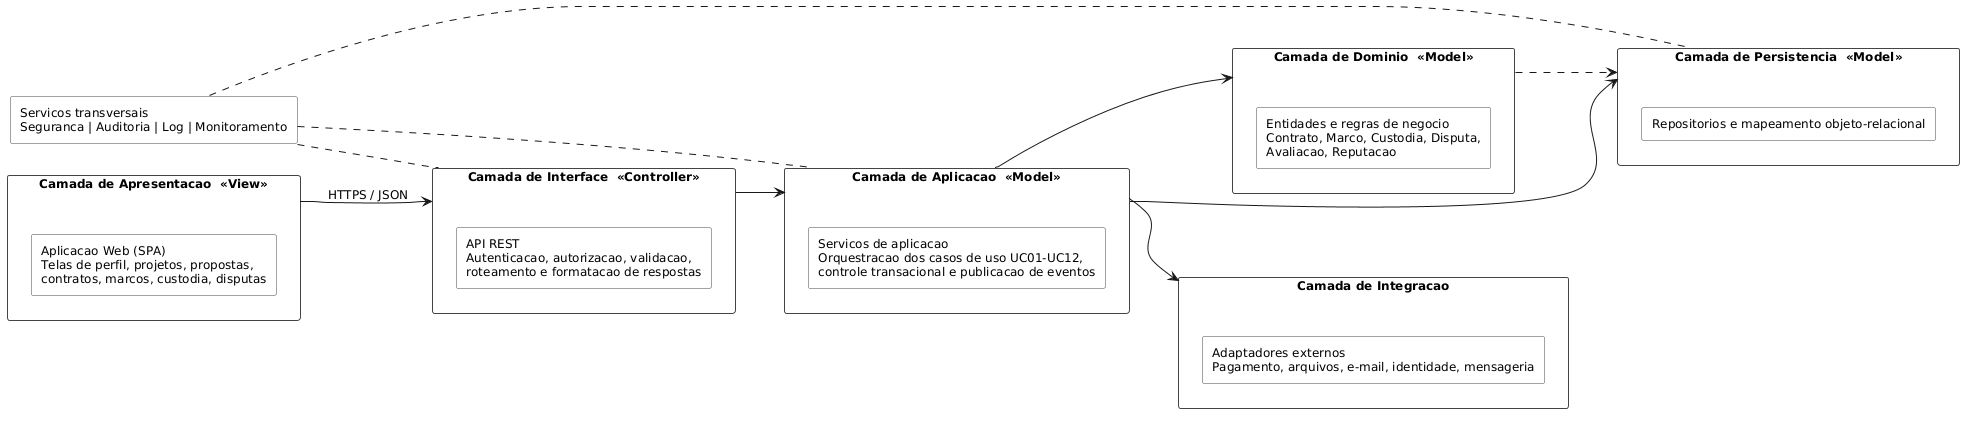
\includegraphics[width=0.8\textwidth]{arquitetura_camadas.png}
\caption{Arquitetura em camadas do DevMatch com a distribuição dos
elementos do padrão MVC.}
\label{fig:arquitetura}
\end{figure*}

A Tabela~\ref{tab:camadas} descreve as responsabilidades de cada
camada e os principais elementos nela alocados.

\begin{table*}[!ht]
\caption{Camadas da arquitetura do DevMatch.}
\label{tab:camadas}
\centering

\begin{tblr}{
    width=\textwidth,
    colspec={
        Q[l,wd=0.18\textwidth]
        Q[l,wd=0.30\textwidth]
        X[l]
    },
    row{1}={
        font=\bfseries,
        bg=gray!15
    },
    cells={
        valign=m,
        font=\scriptsize
    },
    hlines,
    vlines
}

Camada & Responsabilidade & Elementos principais \\

Apresentação &
Exibir as informações ao usuário, capturar suas ações e validar dados
de formulário. Não contém regras de negócio. &
Telas de perfil, busca de projetos, propostas, contratos, marcos,
custódia, disputas e avaliações; componentes de interface; e
roteamento da aplicação Web. \\

Interface (controle) &
Receber as requisições, autenticar e autorizar o solicitante, validar
os dados de entrada, delegar a execução à camada de aplicação e
formatar a resposta. &
Controladores REST (\textit{ProjectController},
\textit{ProposalController}, \textit{ContractController},
\textit{MilestoneController}, \textit{PaymentController},
\textit{DisputeController}); filtros de autenticação; e tratadores de
erro. \\

Aplicação &
Orquestrar os casos de uso, coordenar objetos de domínio, controlar
transações e publicar eventos de notificação e auditoria. &
Serviços de aplicação correspondentes aos casos de uso UC01 a UC12;
coordenadores de transação; e mapeadores entre objetos de
transferência e entidades. \\

Domínio &
Concentrar as entidades, os objetos de valor e as regras de negócio do
sistema, incluindo as máquinas de estado e as invariantes. &
Entidades \textit{Usuario}, \textit{Freelancer}, \textit{Cliente},
\textit{Projeto}, \textit{Proposta}, \textit{Contrato},
\textit{Marco}, \textit{Entrega}, \textit{Custodia},
\textit{Transacao}, \textit{Disputa} e \textit{Avaliacao}; e as regras
de reputação, de liberação de pagamento e de prazo de aprovação. \\

Persistência &
Isolar o acesso aos dados, traduzindo objetos de domínio em registros
do banco de dados e vice-versa. &
Repositórios por agregado; mapeamento objeto-relacional; consultas de
busca e filtragem; e controle de versão do esquema. \\

Integração &
Encapsular a comunicação com sistemas externos, oferecendo interfaces
estáveis ao restante do sistema. &
Adaptadores de gateway de pagamento, de armazenamento de arquivos, de
envio de mensagens e de provedor de identidade; e tratamento de
\textit{webhooks}. \\

Transversal &
Prover funcionalidades utilizadas por várias camadas, sem
acoplá-las a implementações específicas. &
Controle de acesso baseado em papéis, criptografia, registro de
auditoria, log estruturado e monitoramento. \\

\end{tblr}
\end{table*}

O padrão MVC é aplicado sobre essa estrutura conforme apresentado na
Tabela~\ref{tab:mvc}. Adota-se a variante em que a camada de
apresentação executa no cliente e consome uma API REST, de modo que a
\textit{View} é implementada na aplicação Web, o \textit{Controller}
corresponde aos controladores da camada de interface e o \textit{Model}
é formado pelas camadas de aplicação, domínio e persistência.

\begin{table}[!ht]
\caption{Correspondência entre os elementos do MVC e as camadas da
arquitetura.}
\label{tab:mvc}
\centering

\begin{tblr}{
    width=\columnwidth,
    colspec={
        Q[l,wd=0.16\columnwidth]
        Q[l,wd=0.26\columnwidth]
        X[l]
    },
    row{1}={
        font=\bfseries,
        bg=gray!15
    },
    cells={
        valign=m,
        font=\scriptsize
    },
    hlines,
    vlines
}

Elemento & Camada correspondente & Responsabilidade no DevMatch \\

View &
Apresentação &
Renderizar projetos, propostas, contratos, marcos e disputas;
capturar as ações do usuário; e apresentar mensagens de validação e de
confirmação. \\

Controller &
Interface &
Interpretar a requisição, verificar autenticação e permissões,
acionar o serviço de aplicação correspondente e devolver a
representação adequada. \\

Model &
Aplicação, domínio e persistência &
Executar as regras de negócio, manter o estado das entidades,
garantir as invariantes e persistir as alterações. \\

\end{tblr}
\end{table}

A separação entre \textit{Controller} e \textit{Model} é relevante para
os requisitos de segurança e auditoria. Operações sensíveis, como a
liberação de um valor em custódia ou o registro da decisão de uma
disputa, são executadas exclusivamente por serviços da camada de
aplicação, que registram o autor, o instante e o motivo da operação.
Dessa forma, nenhuma alteração financeira depende de validações
realizadas apenas na interface do usuário.

As principais decisões arquiteturais e suas justificativas estão
resumidas na Tabela~\ref{tab:decisoes}.

\begin{table*}[!ht]
\caption{Decisões arquiteturais do DevMatch.}
\label{tab:decisoes}
\centering

\begin{tblr}{
    width=\textwidth,
    colspec={
        Q[l,wd=0.24\textwidth]
        Q[l,wd=0.26\textwidth]
        X[l]
    },
    row{1}={
        font=\bfseries,
        bg=gray!15
    },
    cells={
        valign=m,
        font=\scriptsize
    },
    hlines,
    vlines
}

Decisão & Justificativa & Consequência \\

Arquitetura em camadas com dependência unidirecional &
Isolar as regras de negócio da tecnologia de interface e de
persistência. &
Aumenta a testabilidade e permite substituir a interface ou o
mecanismo de armazenamento com impacto restrito. \\

Padrão MVC na interação com o usuário &
Separar a exibição dos dados do tratamento das requisições em um
sistema com muitos formulários e listagens. &
Facilita a reutilização da API por diferentes clientes, incluindo um
futuro aplicativo móvel. \\

API REST sobre HTTPS &
Padronizar a comunicação entre o cliente e o servidor e permitir
integração com terceiros. &
Exige versionamento da API e tratamento explícito de erros. \\

Custódia implementada como componente próprio, integrado por adaptador &
Concentrar as regras de bloqueio e liberação de valores e evitar
dependência direta de um fornecedor de pagamento. &
Permite trocar o gateway sem alterar as regras de negócio, mas exige
conciliação entre os registros internos e os do provedor. \\

Registro de auditoria transversal e imutável &
Atender aos requisitos de rastreabilidade das alterações contratuais e
das transações financeiras. &
Aumenta o volume de dados armazenados e demanda política de retenção. \\

Processamento assíncrono de notificações e de recomendações &
Evitar que operações demoradas afetem o tempo de resposta das
requisições do usuário. &
Introduz um intermediário de mensagens e exige tratamento de falhas e
de reprocessamento. \\

\end{tblr}
\end{table*}

% ============================================================
% 4.2 DIAGRAMAS DE COMPONENTES E DE IMPLANTAÇÃO
% ============================================================

\subsection{Diagramas de Componentes e de Implantação}
\label{subsec:componentes-implantacao}

\subsubsection{Diagrama de Componentes}
\label{subsubsec:componentes}

O diagrama de componentes representa a decomposição do sistema em
unidades substituíveis e as interfaces por meio das quais essas
unidades se relacionam \citep{omguml}. A Figura~\ref{fig:componentes}
apresenta os componentes do DevMatch, agrupados segundo as camadas
definidas na Seção~\ref{subsec:arquitetura}.

\begin{figure*}[!ht]
\centering
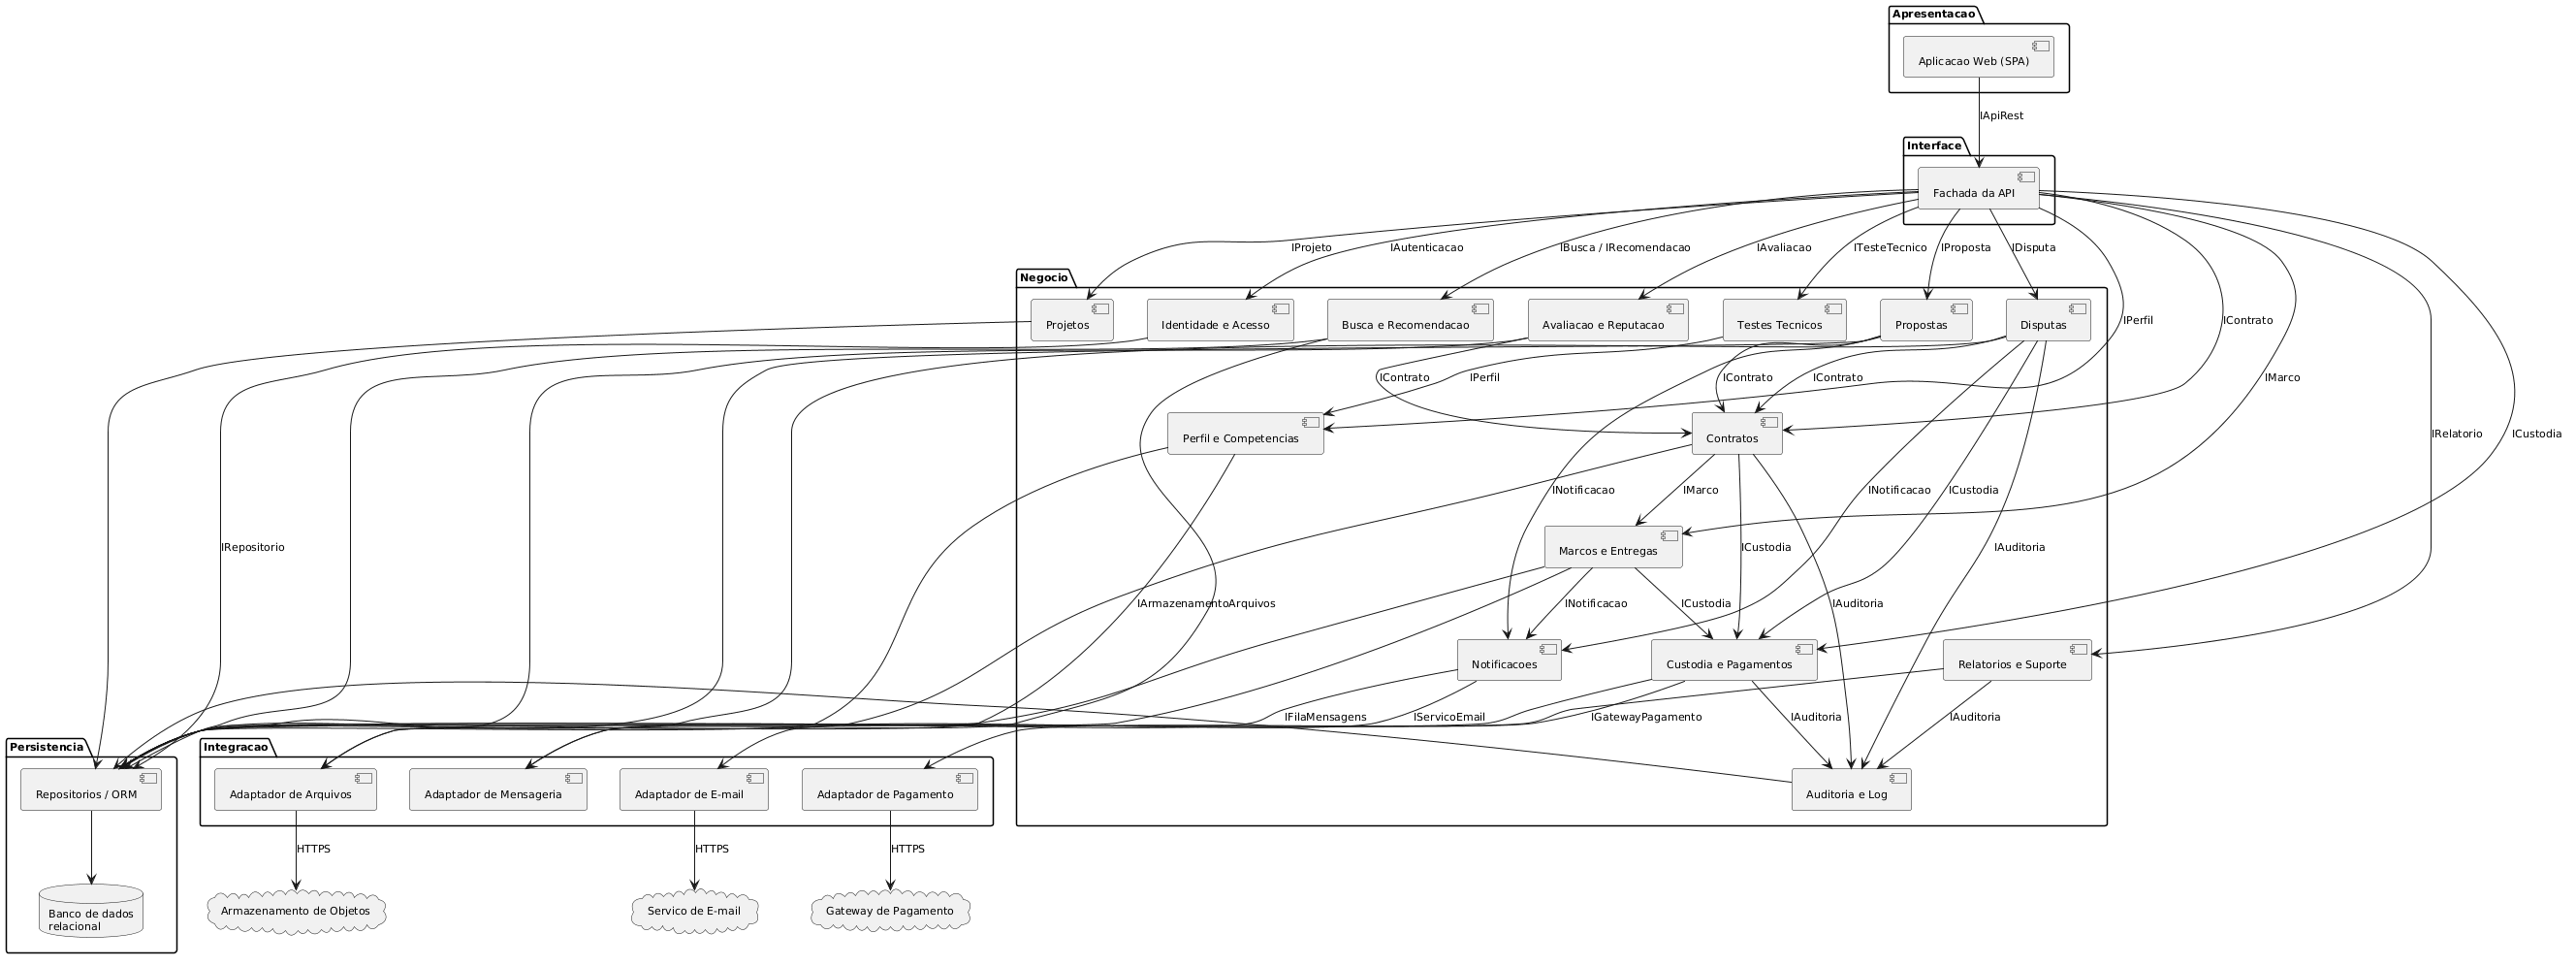
\includegraphics[width=\textwidth]{diagrama_componentes.png}
\caption{Diagrama de componentes do DevMatch. As interfaces fornecidas
são representadas por círculos e as interfaces requeridas por
soquetes.}
\label{fig:componentes}
\end{figure*}

A aplicação Web é o componente cliente e consome a interface
\textit{IApiRest}, exposta pelo componente de fachada da API. Esse
componente concentra a autenticação, o controle de acesso, o
roteamento das requisições e a limitação de taxa, delegando a execução
aos componentes de negócio. Cada componente de negócio corresponde a
um conjunto coeso de casos de uso e fornece uma interface explícita,
o que reduz o acoplamento entre eles e permite sua evolução
independente.

Os componentes de negócio não acessam o banco de dados diretamente.
O acesso ocorre por meio do componente de persistência, que fornece a
interface \textit{IRepositorio} e concentra o mapeamento
objeto-relacional. De modo análogo, a comunicação com serviços
externos é realizada pelos adaptadores da camada de integração, que
isolam as particularidades de cada fornecedor. O componente de
custódia e pagamentos, por exemplo, requer a interface
\textit{IGatewayPagamento}, implementada por um adaptador específico;
a substituição do provedor de pagamento exige apenas a troca desse
adaptador.

A Tabela~\ref{tab:componentes} descreve os componentes, os casos de
uso atendidos e as interfaces fornecidas e requeridas.

\begin{table*}[!ht]
\caption{Componentes do DevMatch, casos de uso atendidos e interfaces.}
\label{tab:componentes}
\centering

\begin{tblr}{
    width=\textwidth,
    colspec={
        Q[l,wd=0.19\textwidth]
        Q[c,wd=0.09\textwidth]
        Q[l,wd=0.32\textwidth]
        X[l]
    },
    row{1}={
        font=\bfseries,
        bg=gray!15
    },
    cells={
        valign=m,
        font=\scriptsize
    },
    hlines,
    vlines
}

Componente & Casos de uso & Responsabilidade & Interfaces \\

Aplicação Web (SPA) &
UC01--UC12 &
Apresentar as telas do sistema e tratar a interação do usuário. &
Requer \textit{IApiRest}. \\

Fachada da API &
UC01--UC12 &
Autenticar as requisições, aplicar o controle de acesso por papel,
rotear as chamadas e padronizar as respostas. &
Fornece \textit{IApiRest}; requer as interfaces dos componentes de
negócio e \textit{IAutenticacao}. \\

Identidade e acesso &
UC10 &
Gerenciar contas, credenciais, papéis, verificação de identidade e
bloqueio de usuários. &
Fornece \textit{IAutenticacao} e \textit{IGestaoUsuarios}; requer
\textit{IRepositorio} e \textit{INotificacao}. \\

Perfil e competências &
UC01 &
Manter perfil profissional, portfólio, certificações,
disponibilidade e valor de trabalho. &
Fornece \textit{IPerfil}; requer \textit{IRepositorio} e
\textit{IArmazenamentoArquivos}. \\

Testes técnicos &
UC01 &
Aplicar testes, corrigir respostas, registrar pontuação e conceder
selos de competência. &
Fornece \textit{ITesteTecnico}; requer \textit{IRepositorio} e
\textit{IPerfil}. \\

Projetos &
UC04 &
Publicar, editar, pausar e encerrar projetos e disponibilizá-los para
busca. &
Fornece \textit{IProjeto}; requer \textit{IRepositorio} e
\textit{IBusca}. \\

Busca e recomendação &
UC02 &
Indexar projetos e perfis, executar consultas com filtros e gerar
sugestões com base em tecnologias, disponibilidade, reputação e faixa
de preço. &
Fornece \textit{IBusca} e \textit{IRecomendacao}; requer
\textit{IRepositorio} e \textit{IFilaMensagens}. \\

Propostas &
UC03, UC05 &
Registrar propostas, manter o histórico de negociação e tratar o
aceite ou a recusa. &
Fornece \textit{IProposta}; requer \textit{IProjeto},
\textit{IContrato}, \textit{IRepositorio} e \textit{INotificacao}. \\

Contratos &
UC06 &
Gerar o contrato a partir da proposta aceita, controlar a confirmação
das partes e a máquina de estados do contrato. &
Fornece \textit{IContrato}; requer \textit{IMarco},
\textit{ICustodia}, \textit{IRepositorio} e \textit{IAuditoria}. \\

Marcos e entregas &
UC07 &
Definir marcos, registrar entregas e artefatos, tratar aprovações,
ajustes e prazos de avaliação. &
Fornece \textit{IMarco}; requer \textit{IArmazenamentoArquivos},
\textit{ICustodia}, \textit{IRepositorio} e \textit{INotificacao}. \\

Custódia e pagamentos &
UC08 &
Registrar depósitos, manter valores bloqueados, liberar repasses,
descontar comissões e tratar estornos e reembolsos. &
Fornece \textit{ICustodia}; requer \textit{IGatewayPagamento},
\textit{IRepositorio} e \textit{IAuditoria}. \\

Disputas &
UC09 &
Registrar disputas e evidências, controlar o fluxo de mediação e
aplicar a decisão sobre os valores em custódia. &
Fornece \textit{IDisputa}; requer \textit{IContrato},
\textit{ICustodia}, \textit{IRepositorio} e \textit{IAuditoria}. \\

Avaliação e reputação &
UC11 &
Registrar avaliações bidirecionais após o encerramento do contrato e
recalcular a reputação. &
Fornece \textit{IAvaliacao}; requer \textit{IContrato} e
\textit{IRepositorio}. \\

Relatórios e suporte &
UC12 &
Consultar transações, gerar relatórios financeiros e de comissões e
tratar chamados. &
Fornece \textit{IRelatorio}; requer \textit{IRepositorio} e
\textit{IAuditoria}. \\

Auditoria e log &
UC09, UC10 &
Registrar de forma imutável as operações sensíveis, os acessos e as
alterações contratuais e financeiras. &
Fornece \textit{IAuditoria}; requer \textit{IRepositorio}. \\

Notificações &
UC03--UC09 &
Enviar mensagens por correio eletrônico e notificações internas a
partir de eventos do sistema. &
Fornece \textit{INotificacao}; requer \textit{IFilaMensagens} e
\textit{IServicoEmail}. \\

Persistência &
--- &
Concentrar o acesso aos dados e o mapeamento objeto-relacional. &
Fornece \textit{IRepositorio}; requer o driver do banco de dados. \\

Adaptadores de integração &
--- &
Encapsular a comunicação com gateway de pagamento, armazenamento de
objetos, serviço de correio eletrônico e intermediário de mensagens. &
Fornecem \textit{IGatewayPagamento},
\textit{IArmazenamentoArquivos}, \textit{IServicoEmail} e
\textit{IFilaMensagens}. \\

\end{tblr}
\end{table*}

\subsubsection{Diagrama de Implantação}
\label{subsubsec:implantacao}

O diagrama de implantação descreve a distribuição física dos
artefatos de software nos nós de execução e os protocolos de
comunicação entre eles \citep{omguml}. A Figura~\ref{fig:implantacao}
apresenta a topologia prevista para o DevMatch.

\begin{figure*}[!ht]
\centering
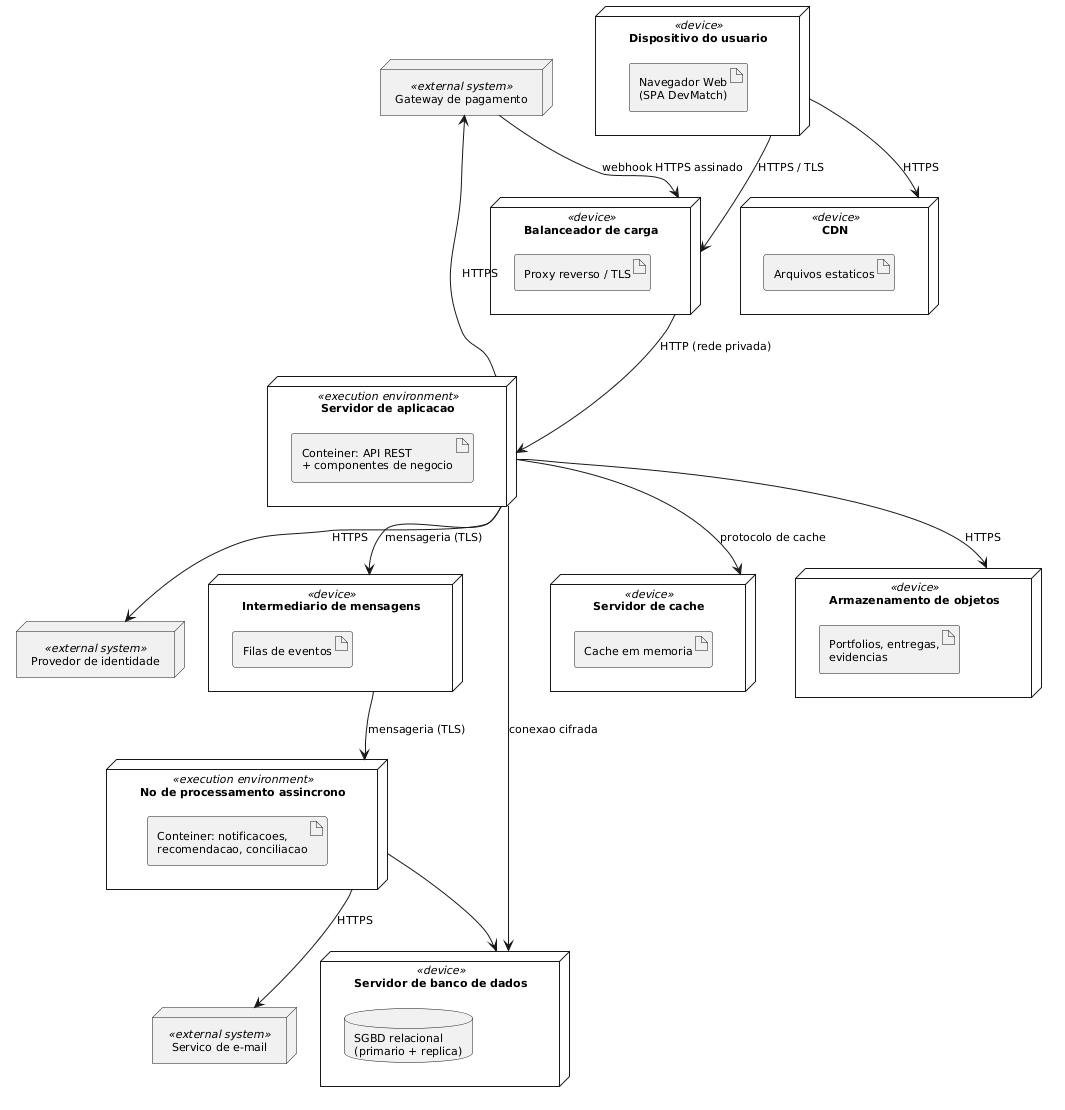
\includegraphics[width=0.8\textwidth]{diagrama_implantacao.png}
\caption{Diagrama de implantação do DevMatch.}
\label{fig:implantacao}
\end{figure*}

O usuário acessa a plataforma por meio de um navegador Web, que obtém
os artefatos estáticos da aplicação a partir de uma rede de
distribuição de conteúdo. As requisições dinâmicas são encaminhadas ao
balanceador de carga, responsável por encerrar a conexão segura e
distribuir as chamadas entre as instâncias do servidor de aplicação.
Essas instâncias executam em contêineres e não mantêm estado de
sessão, o que permite a escalabilidade horizontal do sistema conforme
a demanda.

O servidor de aplicação comunica-se com o servidor de banco de dados
relacional, configurado com uma instância primária para escrita e uma
réplica para leitura e para a geração de relatórios. O servidor de
cache armazena resultados de consultas frequentes, listas de
recomendação e dados de sessão de curta duração. Os artefatos enviados
pelos freelancers, bem como as evidências anexadas às disputas, são
armazenados em um serviço de armazenamento de objetos, e não no
sistema de arquivos do servidor de aplicação. As tarefas assíncronas,
como o envio de notificações, o recálculo de recomendações e a
conciliação financeira, são executadas por nós de processamento
próprios, acionados por um intermediário de mensagens.

Os serviços externos são representados como nós distintos. O gateway
de pagamento é acessado por meio de chamadas HTTPS e informa a
confirmação das operações por \textit{webhooks}, recebidos por um
endereço específico da API e validados por assinatura. Toda a
comunicação externa utiliza TLS, e as credenciais de acesso aos
serviços são mantidas em um cofre de segredos, fora do código-fonte e
das imagens de contêiner. A Tabela~\ref{tab:implantacao} resume os nós,
os artefatos implantados e os protocolos utilizados.

\begin{table*}[!ht]
\caption{Nós de implantação, artefatos e protocolos de comunicação.}
\label{tab:implantacao}
\centering

\begin{tblr}{
    width=\textwidth,
    colspec={
        Q[l,wd=0.20\textwidth]
        Q[l,wd=0.26\textwidth]
        Q[l,wd=0.20\textwidth]
        X[l]
    },
    row{1}={
        font=\bfseries,
        bg=gray!15
    },
    cells={
        valign=m,
        font=\scriptsize
    },
    hlines,
    vlines
}

Nó & Artefatos & Comunicação & Observações \\

Dispositivo do usuário
\mbox{$\langle\langle$device$\rangle\rangle$} &
Navegador Web com a aplicação de página única. &
HTTPS/TLS com o balanceador e com a rede de distribuição. &
Não armazena dados sensíveis além do token de sessão. \\

Rede de distribuição de conteúdo
\mbox{$\langle\langle$device$\rangle\rangle$} &
Arquivos estáticos da interface. &
HTTPS. &
Reduz a latência de carregamento e o tráfego no servidor de
aplicação. \\

Balanceador de carga
\mbox{$\langle\langle$device$\rangle\rangle$} &
Proxy reverso e terminação TLS. &
HTTPS para o exterior e HTTP interno na rede privada. &
Distribui as requisições e realiza verificação de integridade das
instâncias. \\

Servidor de aplicação
\mbox{$\langle\langle$execution environment$\rangle\rangle$} &
Contêineres com a API REST e os componentes de negócio. &
Protocolo do banco de dados, protocolo de cache, HTTPS para serviços
externos e mensagens assíncronas. &
Instâncias sem estado, replicadas e escaláveis horizontalmente. \\

Nó de processamento assíncrono
\mbox{$\langle\langle$execution environment$\rangle\rangle$} &
Contêineres de tarefas de notificação, recomendação e conciliação. &
Mensagens assíncronas e protocolo do banco de dados. &
Isola tarefas de longa duração das requisições interativas. \\

Intermediário de mensagens
\mbox{$\langle\langle$device$\rangle\rangle$} &
Filas de eventos do sistema. &
Protocolo de mensageria sobre TLS. &
Garante a entrega dos eventos e permite reprocessamento. \\

Servidor de banco de dados
\mbox{$\langle\langle$device$\rangle\rangle$} &
Banco de dados relacional, instância primária e réplica de leitura. &
Conexão autenticada e cifrada na rede privada. &
Armazena dados de usuários, contratos, transações e auditoria; possui
rotina de cópia de segurança. \\

Servidor de cache
\mbox{$\langle\langle$device$\rangle\rangle$} &
Cache em memória. &
Protocolo de cache na rede privada. &
Armazena consultas frequentes e recomendações pré-calculadas. \\

Armazenamento de objetos
\mbox{$\langle\langle$device$\rangle\rangle$} &
Portfólios, artefatos de entrega e evidências de disputa. &
HTTPS com acesso por credencial temporária. &
Mantém versões dos arquivos e registra os acessos. \\

Gateway de pagamento
\mbox{$\langle\langle$external system$\rangle\rangle$} &
Serviço de processamento de pagamentos e custódia. &
HTTPS e \textit{webhooks} assinados. &
Responsável pela movimentação financeira efetiva; o sistema mantém o
registro conciliado das operações. \\

Serviços de correio eletrônico e identidade
\mbox{$\langle\langle$external system$\rangle\rangle$} &
Envio de mensagens e autenticação federada. &
HTTPS. &
Utilizados pelos adaptadores da camada de integração. \\

\end{tblr}
\end{table*}

A topologia apresentada atende aos requisitos não funcionais definidos
para o sistema. A replicação das instâncias de aplicação e do banco de
dados contribui para a disponibilidade; a separação entre requisições
interativas e tarefas assíncronas favorece o desempenho; o uso de TLS,
do cofre de segredos e do registro de auditoria em nó dedicado atende
aos requisitos de segurança e rastreabilidade; e o empacotamento em
contêineres facilita a implantação em diferentes provedores de
infraestrutura.

\subsubsection{Diagrama de Classes}
\label{subsec:classes}

O diagrama de classes do DevMatch representa a estrutura estática das
principais entidades do sistema, seus atributos, operações e
relacionamentos. A modelagem foi construída a partir dos atores,
casos de uso e requisitos identificados na etapa de análise,
buscando manter rastreabilidade entre as funcionalidades especificadas
e as classes responsáveis por realizá-las.

A classe abstrata \texttt{Usuario} concentra informações comuns aos
usuários da plataforma. A partir dela são especializadas as classes
\texttt{Freelancer}, \texttt{Cliente}, \texttt{Administrador} e
\texttt{AnalistaFinanceiroSuporte}, correspondentes aos atores
identificados na modelagem de requisitos.

O freelancer possui informações profissionais e competências,
utilizadas tanto na apresentação de seu perfil quanto no mecanismo
de recomendação de projetos. Os projetos são publicados pelos
clientes e podem possuir requisitos de competências, além de receber
propostas enviadas pelos freelancers.

Quando uma proposta é aceita, ela pode originar um contrato,
responsável por formalizar a relação entre cliente e freelancer.
O contrato pode ser dividido em marcos, que organizam a execução do
projeto em etapas e podem receber entregas realizadas pelo
freelancer.

O gerenciamento financeiro é representado pelo pagamento em custódia,
associado aos marcos do contrato. O valor permanece retido até que
as condições estabelecidas sejam atendidas ou uma eventual disputa
seja resolvida.

O sistema também mantém avaliações dos participantes, registros de
auditoria, chamados de suporte e relatórios financeiros e
operacionais. A Figura~\ref{fig:classes-resumido} apresenta uma visão
simplificada das principais classes e relacionamentos do DevMatch.
A versão completa do diagrama é apresentada no
Apêndice~\ref{ap:classes-completo}.

\begin{figure*}[!ht]
\centering
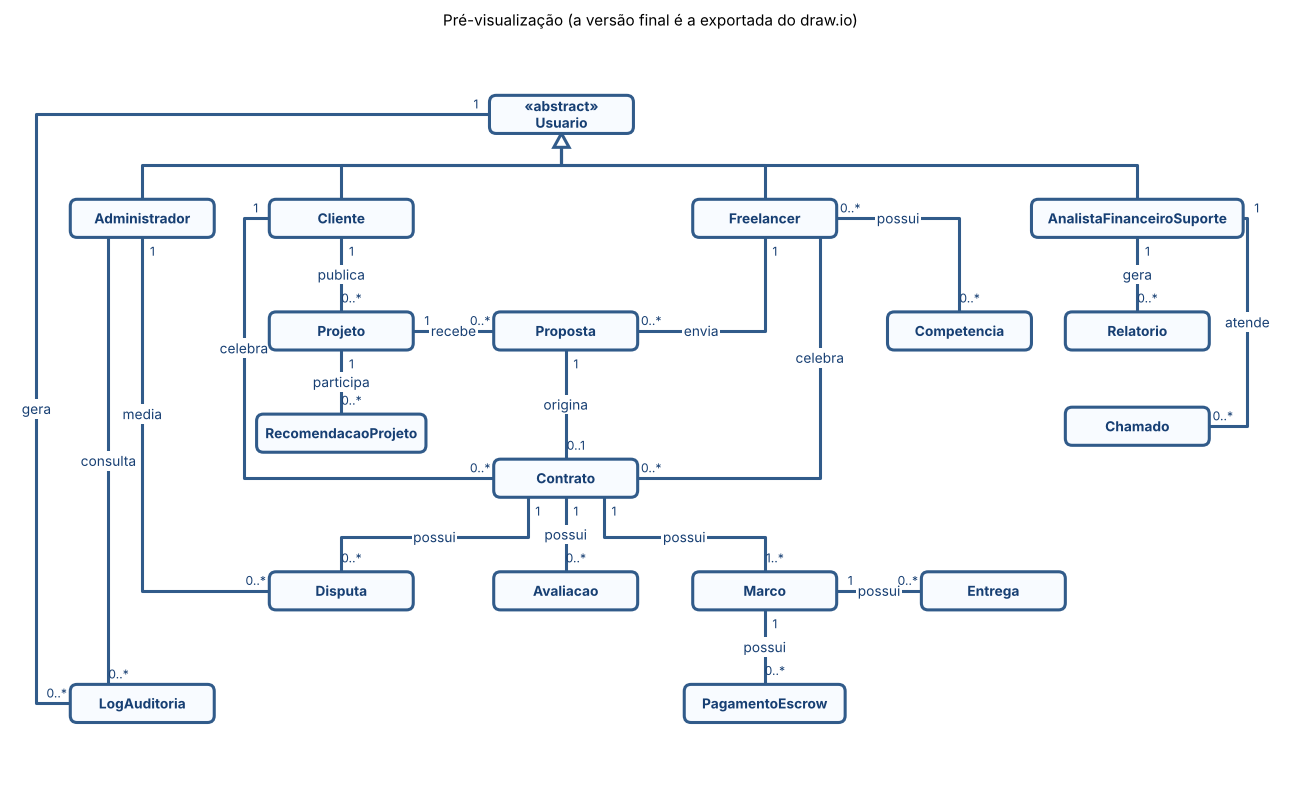
\includegraphics[width=0.8\textwidth]
{diagramas/diagrama_classes_resumido.png}
\caption{Visão resumida do diagrama de classes do DevMatch.}
\label{fig:classes-resumido}
\end{figure*}



\subsection{Diagramas de Sequência}
\label{subsec:sequencia}

% Inserir os diagramas de sequência.

\subsection{Diagramas de Comunicação}
\label{subsec:comunicacao}

% Inserir os diagramas de comunicação.

\subsection{Diagramas de Estados}
\label{subsec:estados}

% Inserir os diagramas de estados.

% ============================================================
% 5 MODELAGEM DE DADOS
% ============================================================

\section{Modelagem de Dados}
\label{sec:modelagem-dados}

% Inserir o modelo conceitual, lógico e físico do banco de dados.

% ============================================================
% 6 CONCLUSÃO
% ============================================================

\section{Conclusão}
\label{sec:conclusao}

% A conclusão deve ser escrita depois da finalização das modelagens.

\appendix

\subsection{Diagrama de Classes Completo}
\label{ap:classes-completo}

A Figura~\ref{fig:classes-completo} apresenta a versão completa do
diagrama de classes do DevMatch, incluindo atributos, operações,
cardinalidades, relações de herança, associações, composições e
tipos enumerados utilizados pela modelagem.

\begin{figure*}[!ht]
\centering
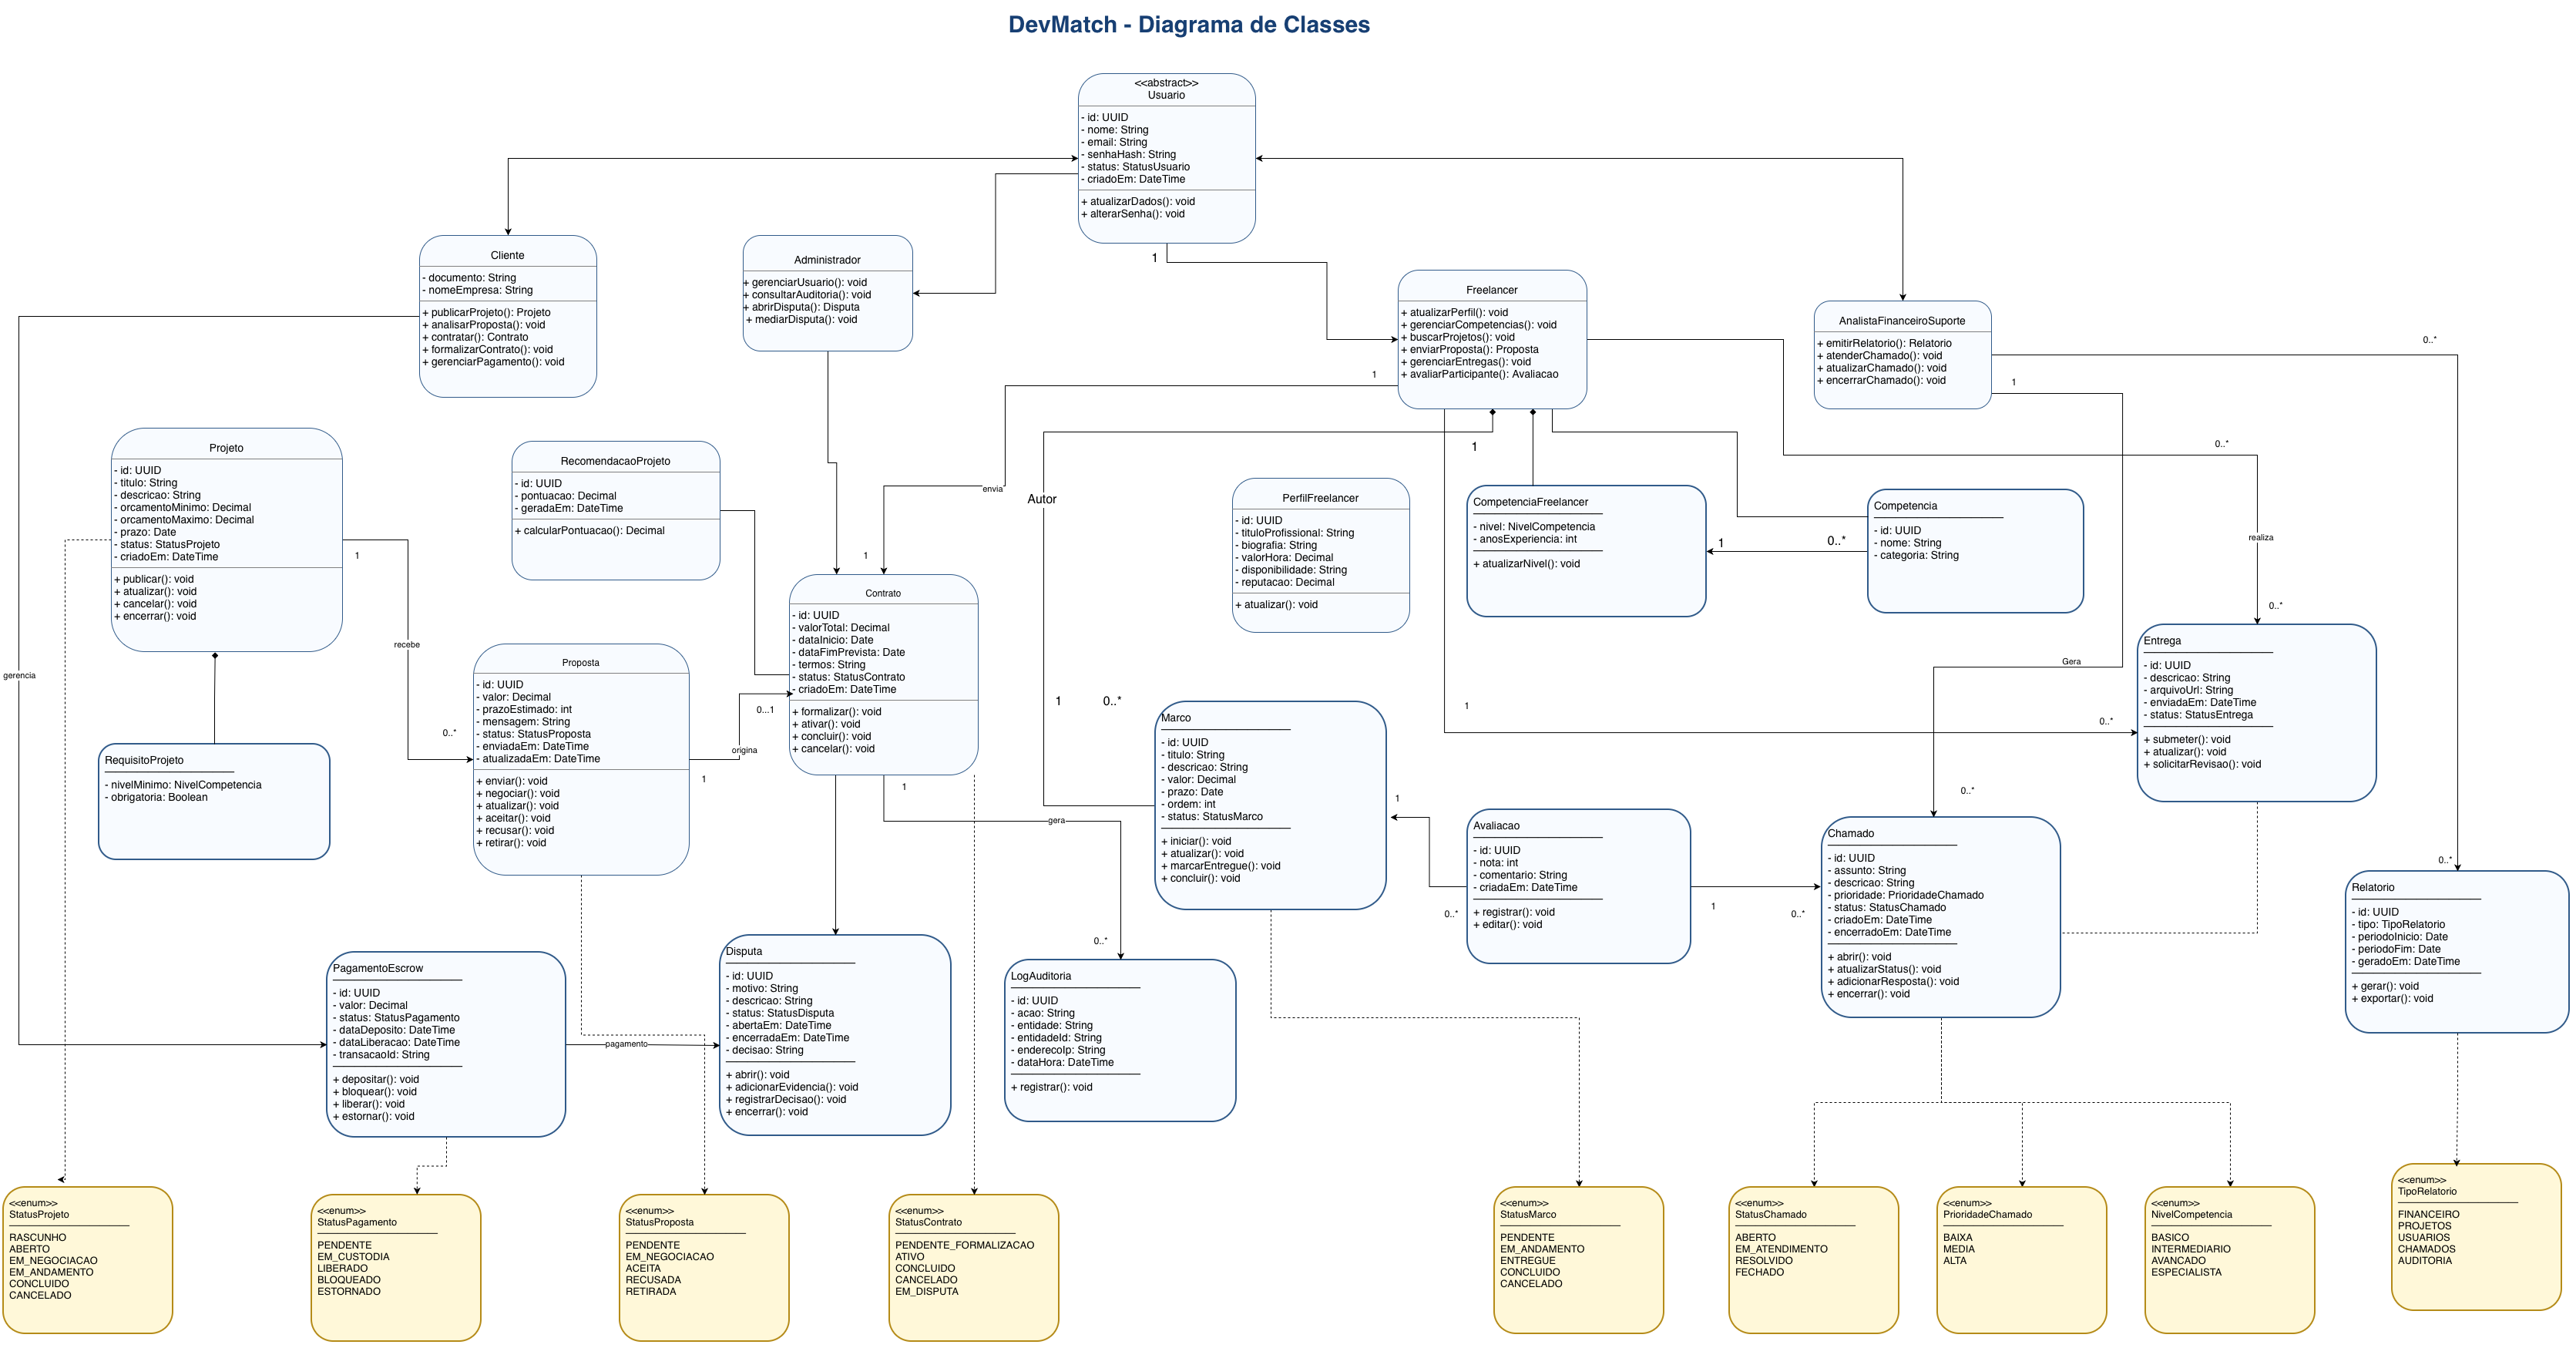
\includegraphics[width=\textwidth]
{diagramas/diagrama_classes_completo.png}
\caption{Diagrama de classes completo do DevMatch.}
\label{fig:classes-completo}
\end{figure*}

% Diagramas e contratos do item 4(c). Incluido por main.tex.
\clearpage
\subsection{Diagramas de Sequência do Sistema}
\label{ap:dss}

As Figuras~\ref{fig:dss-uc03}--\ref{fig:dss-uc09} apresentam as
mensagens observáveis dos seis casos de uso centrais. O serviço de
pagamento é mostrado como ator externo no UC08, sem detalhar a
implementação dos componentes internos do DevMatch.

\begin{figure*}[!p]
\centering
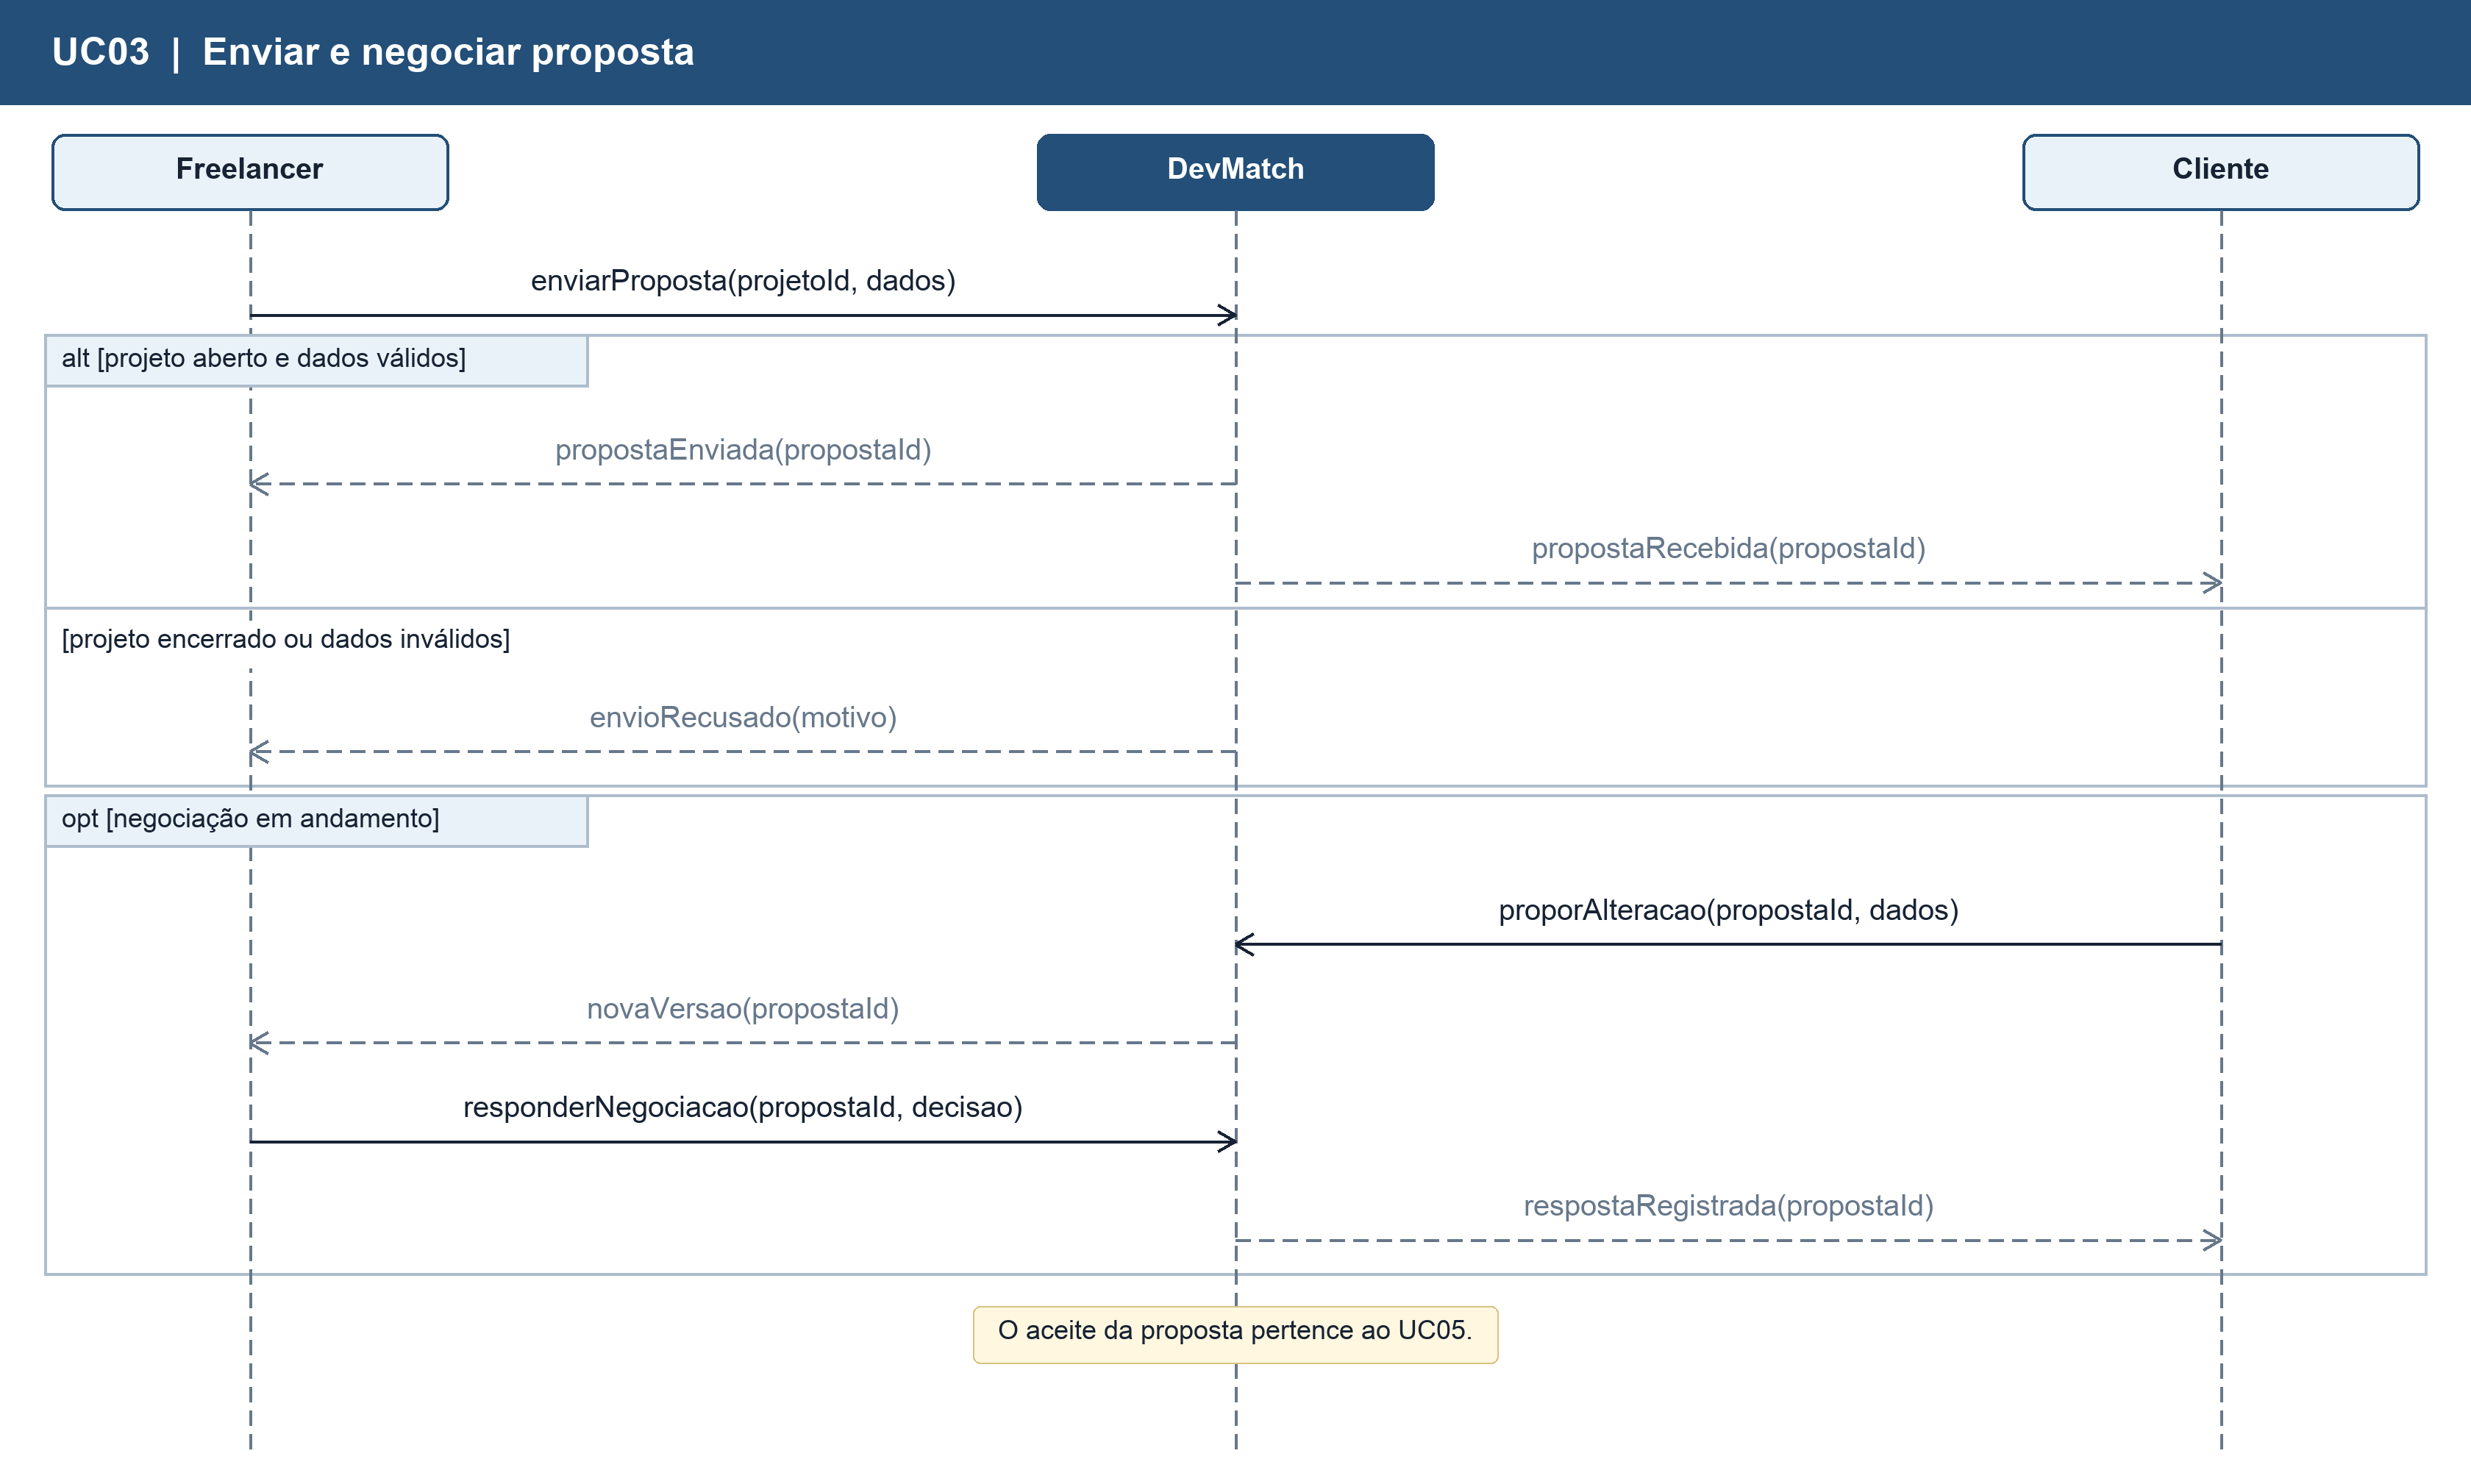
\includegraphics[width=\textwidth,height=0.80\textheight,keepaspectratio]{diagramas/dss_uc03.png}
\caption{DSS do UC03: envio e negociação de proposta.}
\label{fig:dss-uc03}
\end{figure*}

\begin{figure*}[!p]
\centering
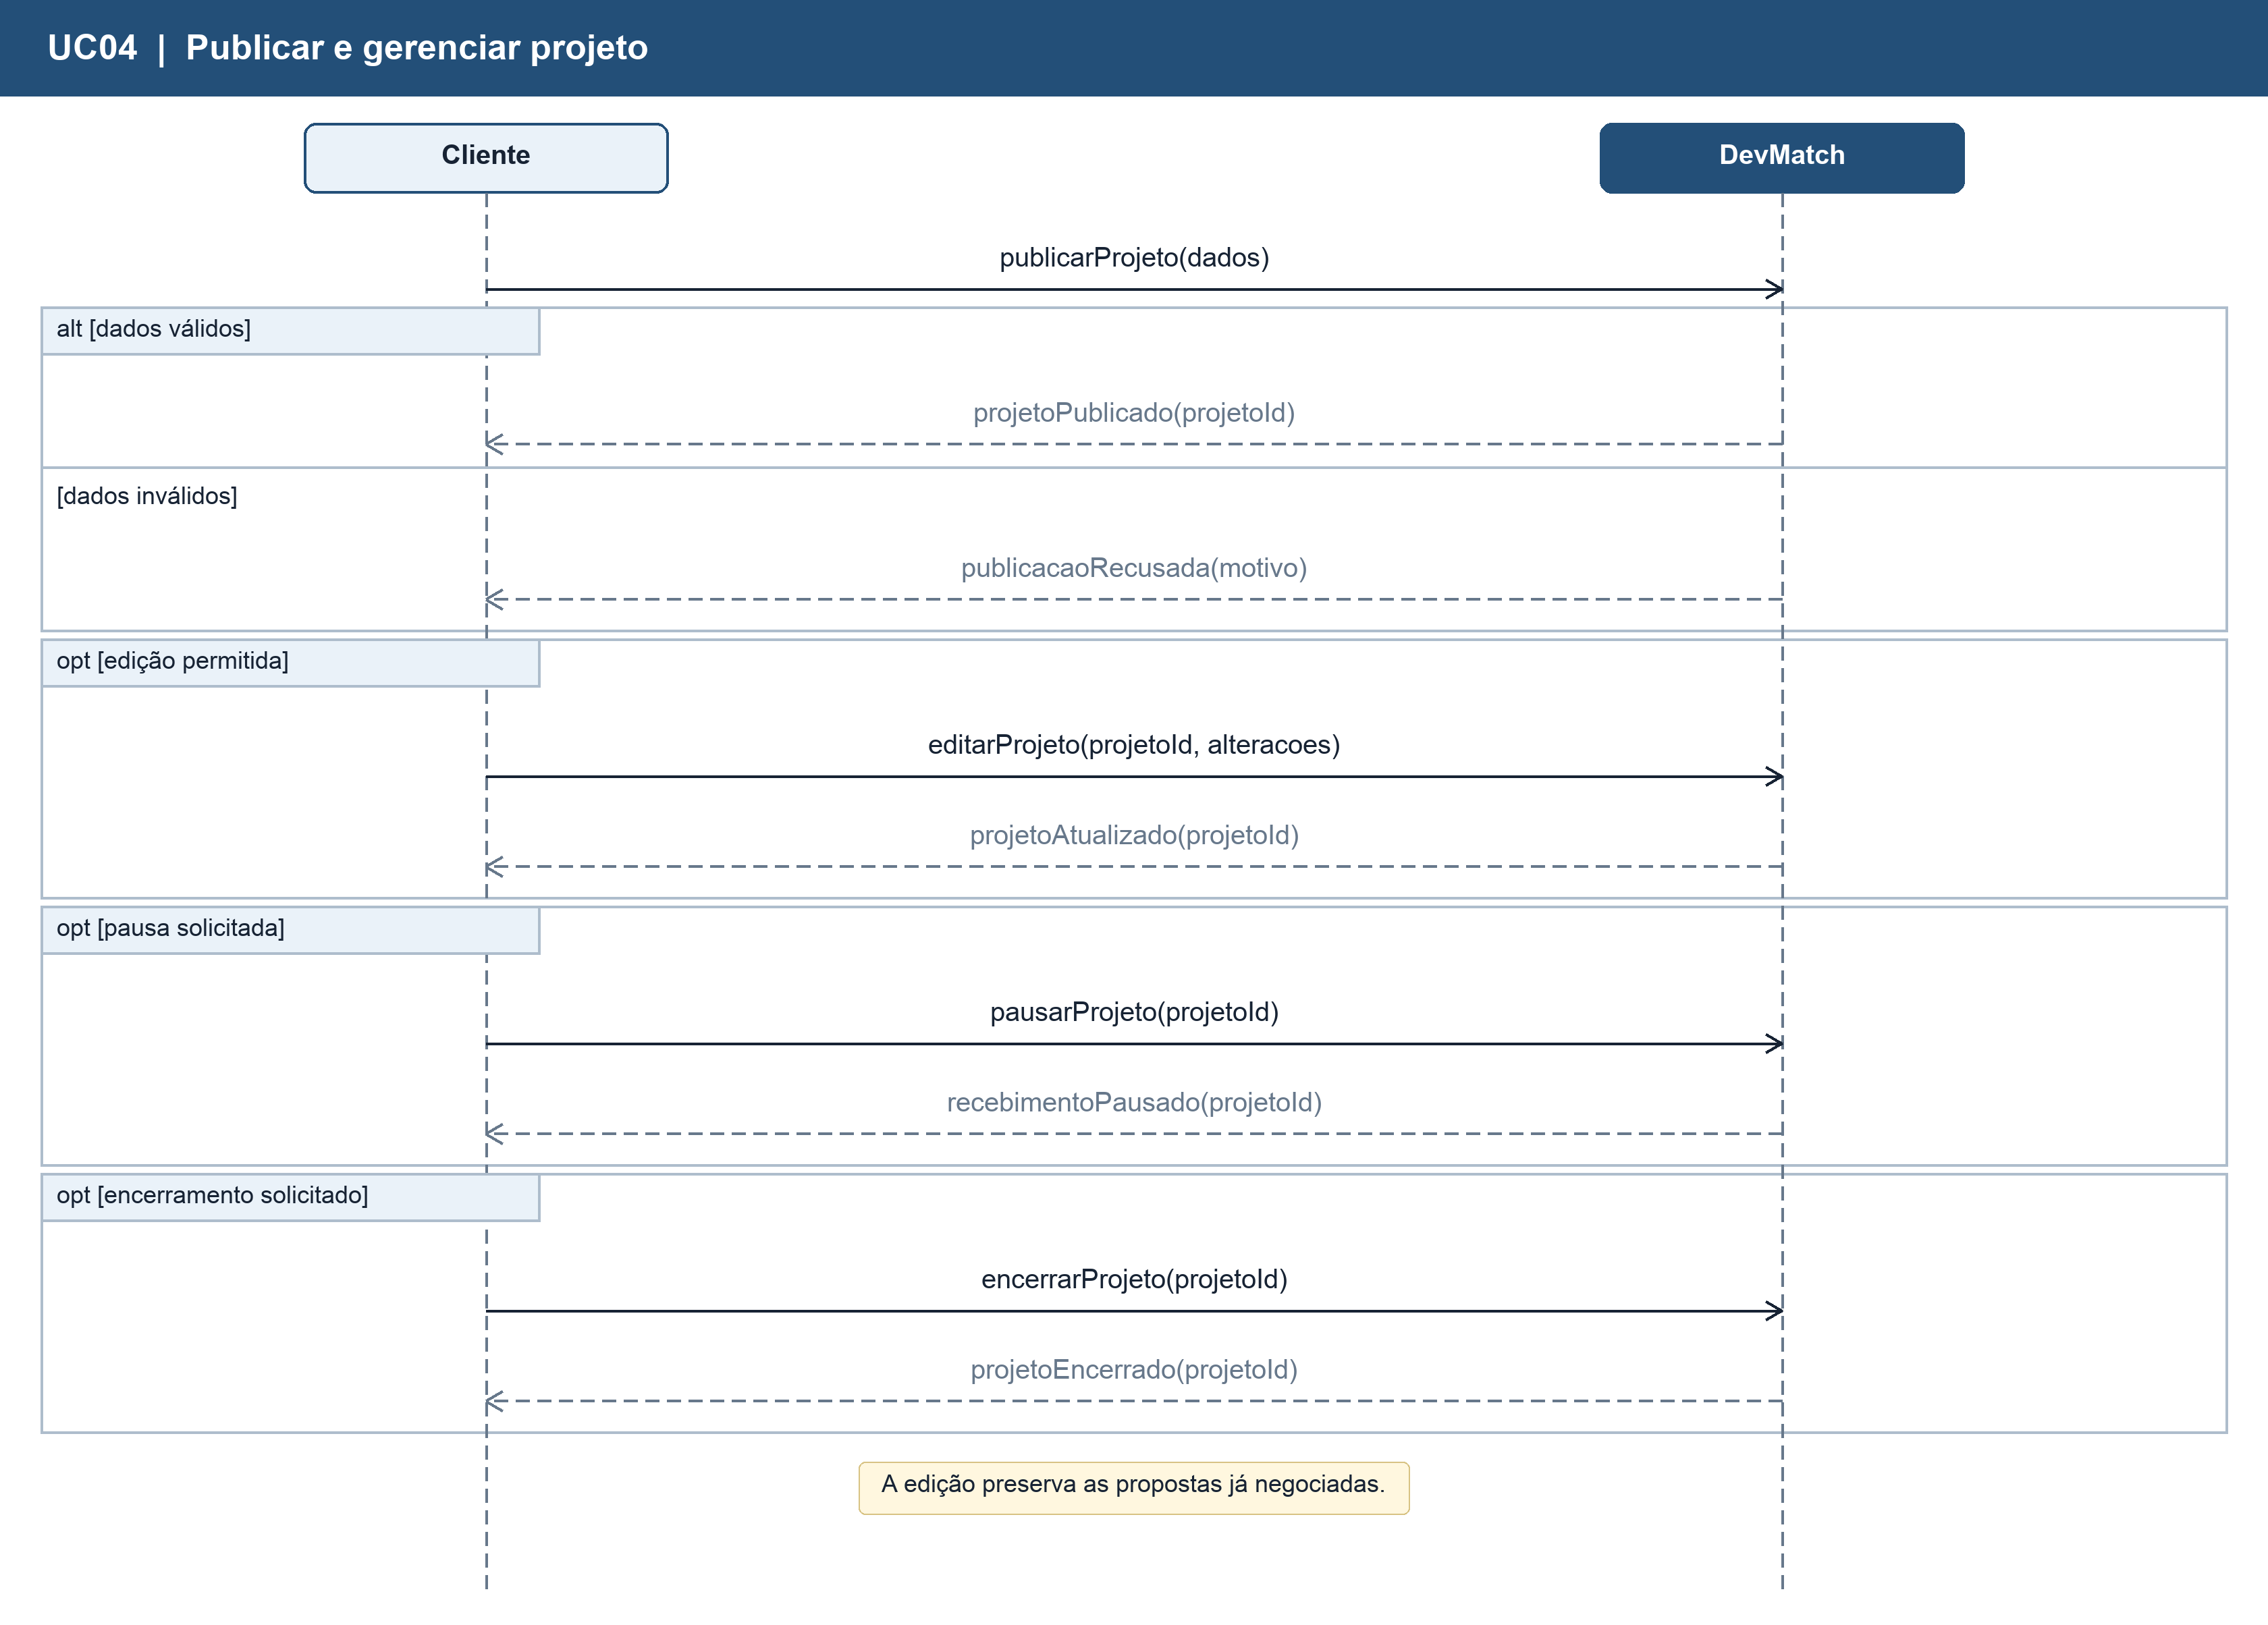
\includegraphics[width=\textwidth,height=0.80\textheight,keepaspectratio]{diagramas/dss_uc04.png}
\caption{DSS do UC04: publicação e gerenciamento de projeto.}
\label{fig:dss-uc04}
\end{figure*}

\begin{figure*}[!p]
\centering
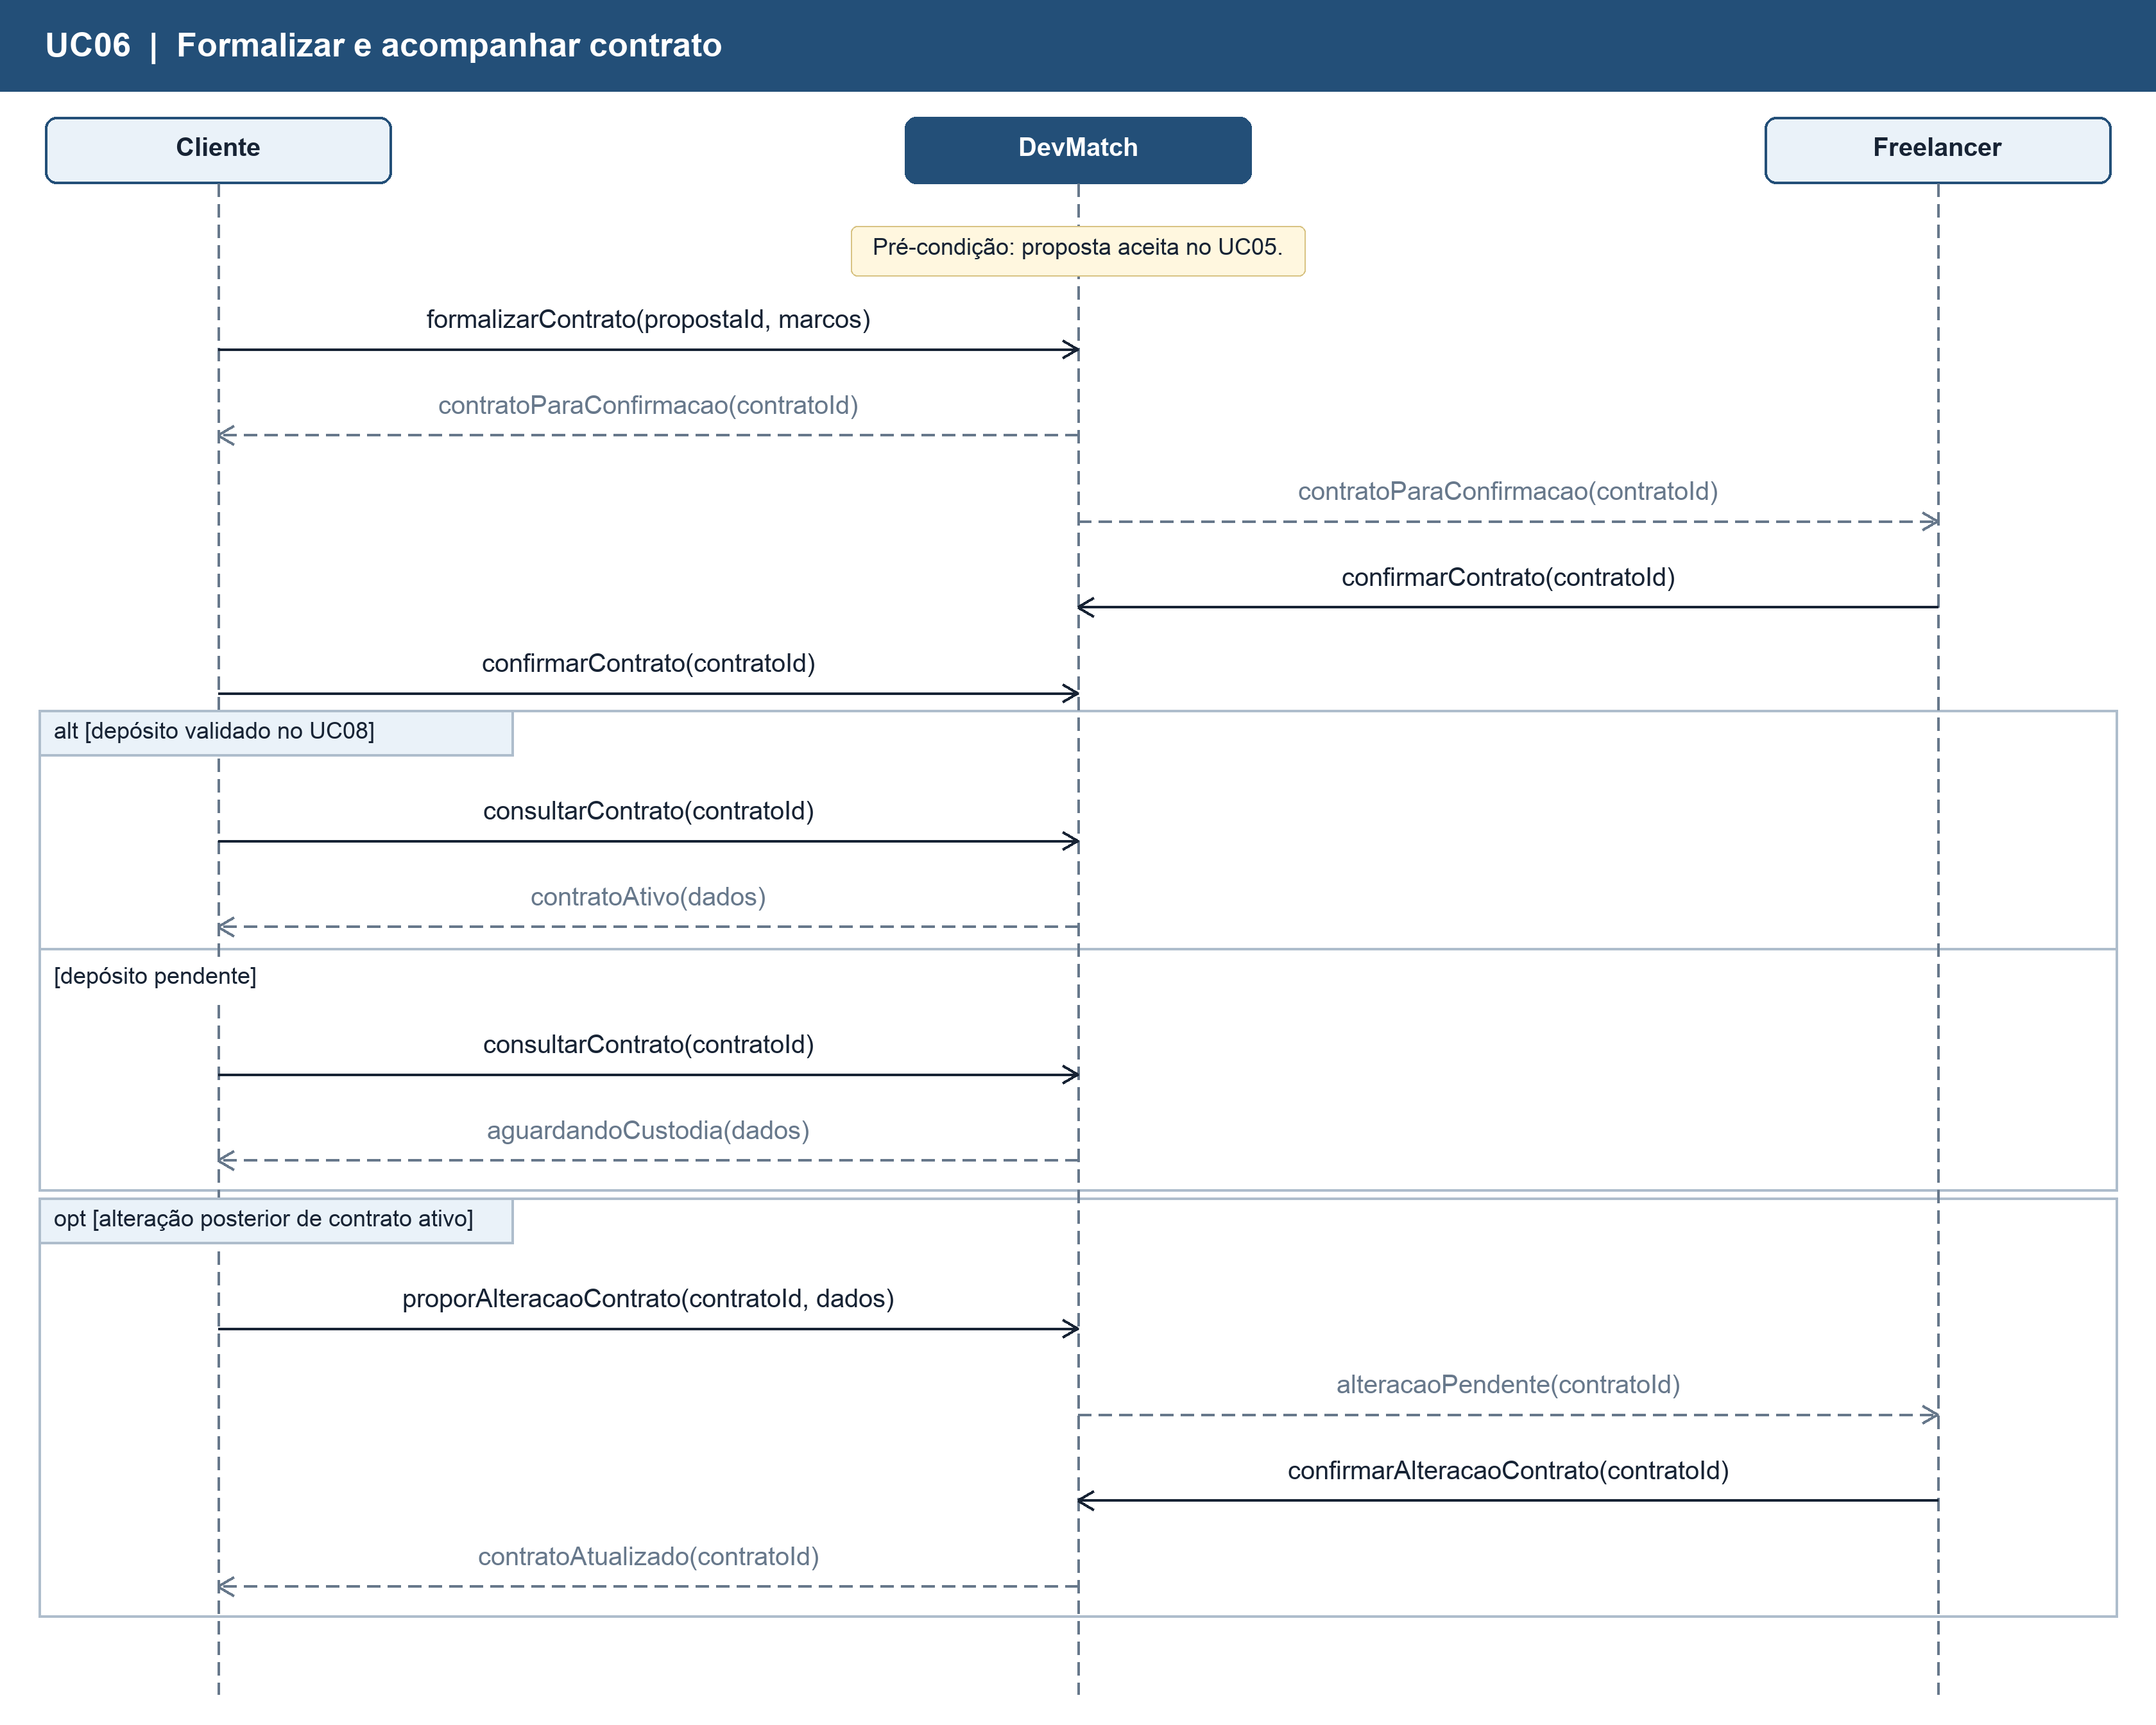
\includegraphics[width=\textwidth,height=0.80\textheight,keepaspectratio]{diagramas/dss_uc06.png}
\caption{DSS do UC06: formalização e acompanhamento de contrato.}
\label{fig:dss-uc06}
\end{figure*}

\begin{figure*}[!p]
\centering
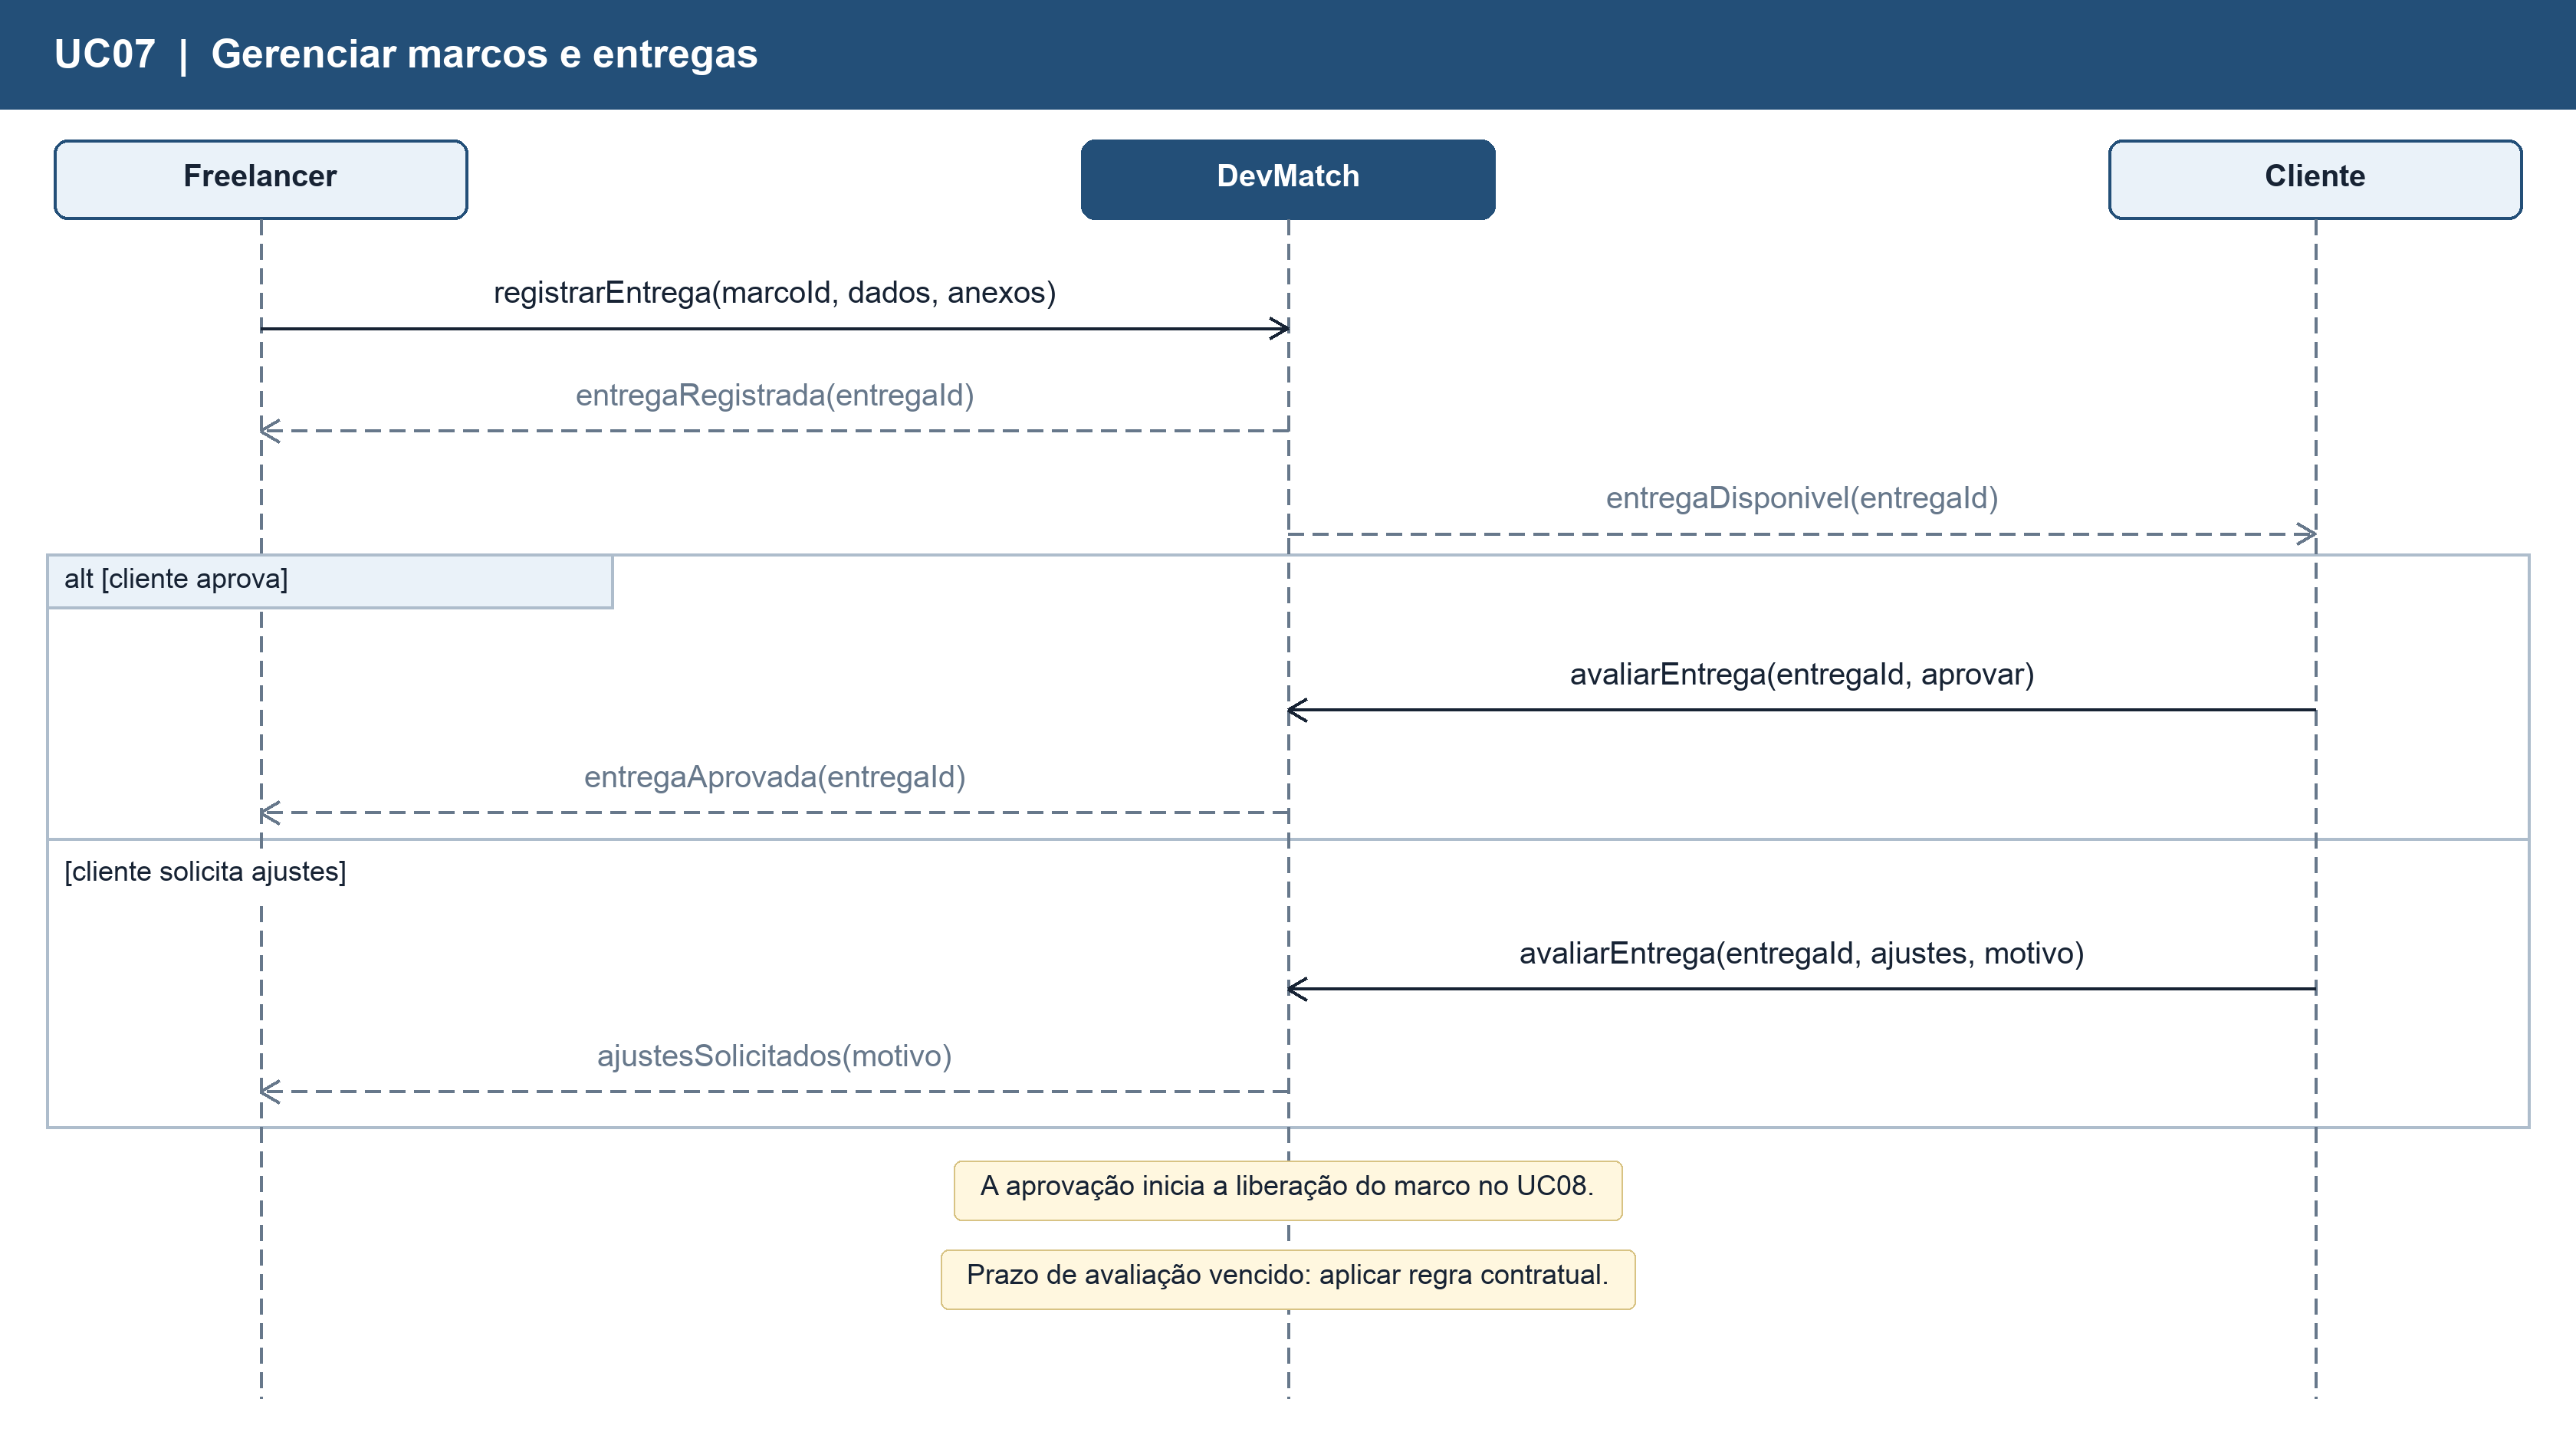
\includegraphics[width=\textwidth,height=0.80\textheight,keepaspectratio]{diagramas/dss_uc07.png}
\caption{DSS do UC07: gerenciamento de marcos e entregas.}
\label{fig:dss-uc07}
\end{figure*}

\begin{figure*}[!p]
\centering
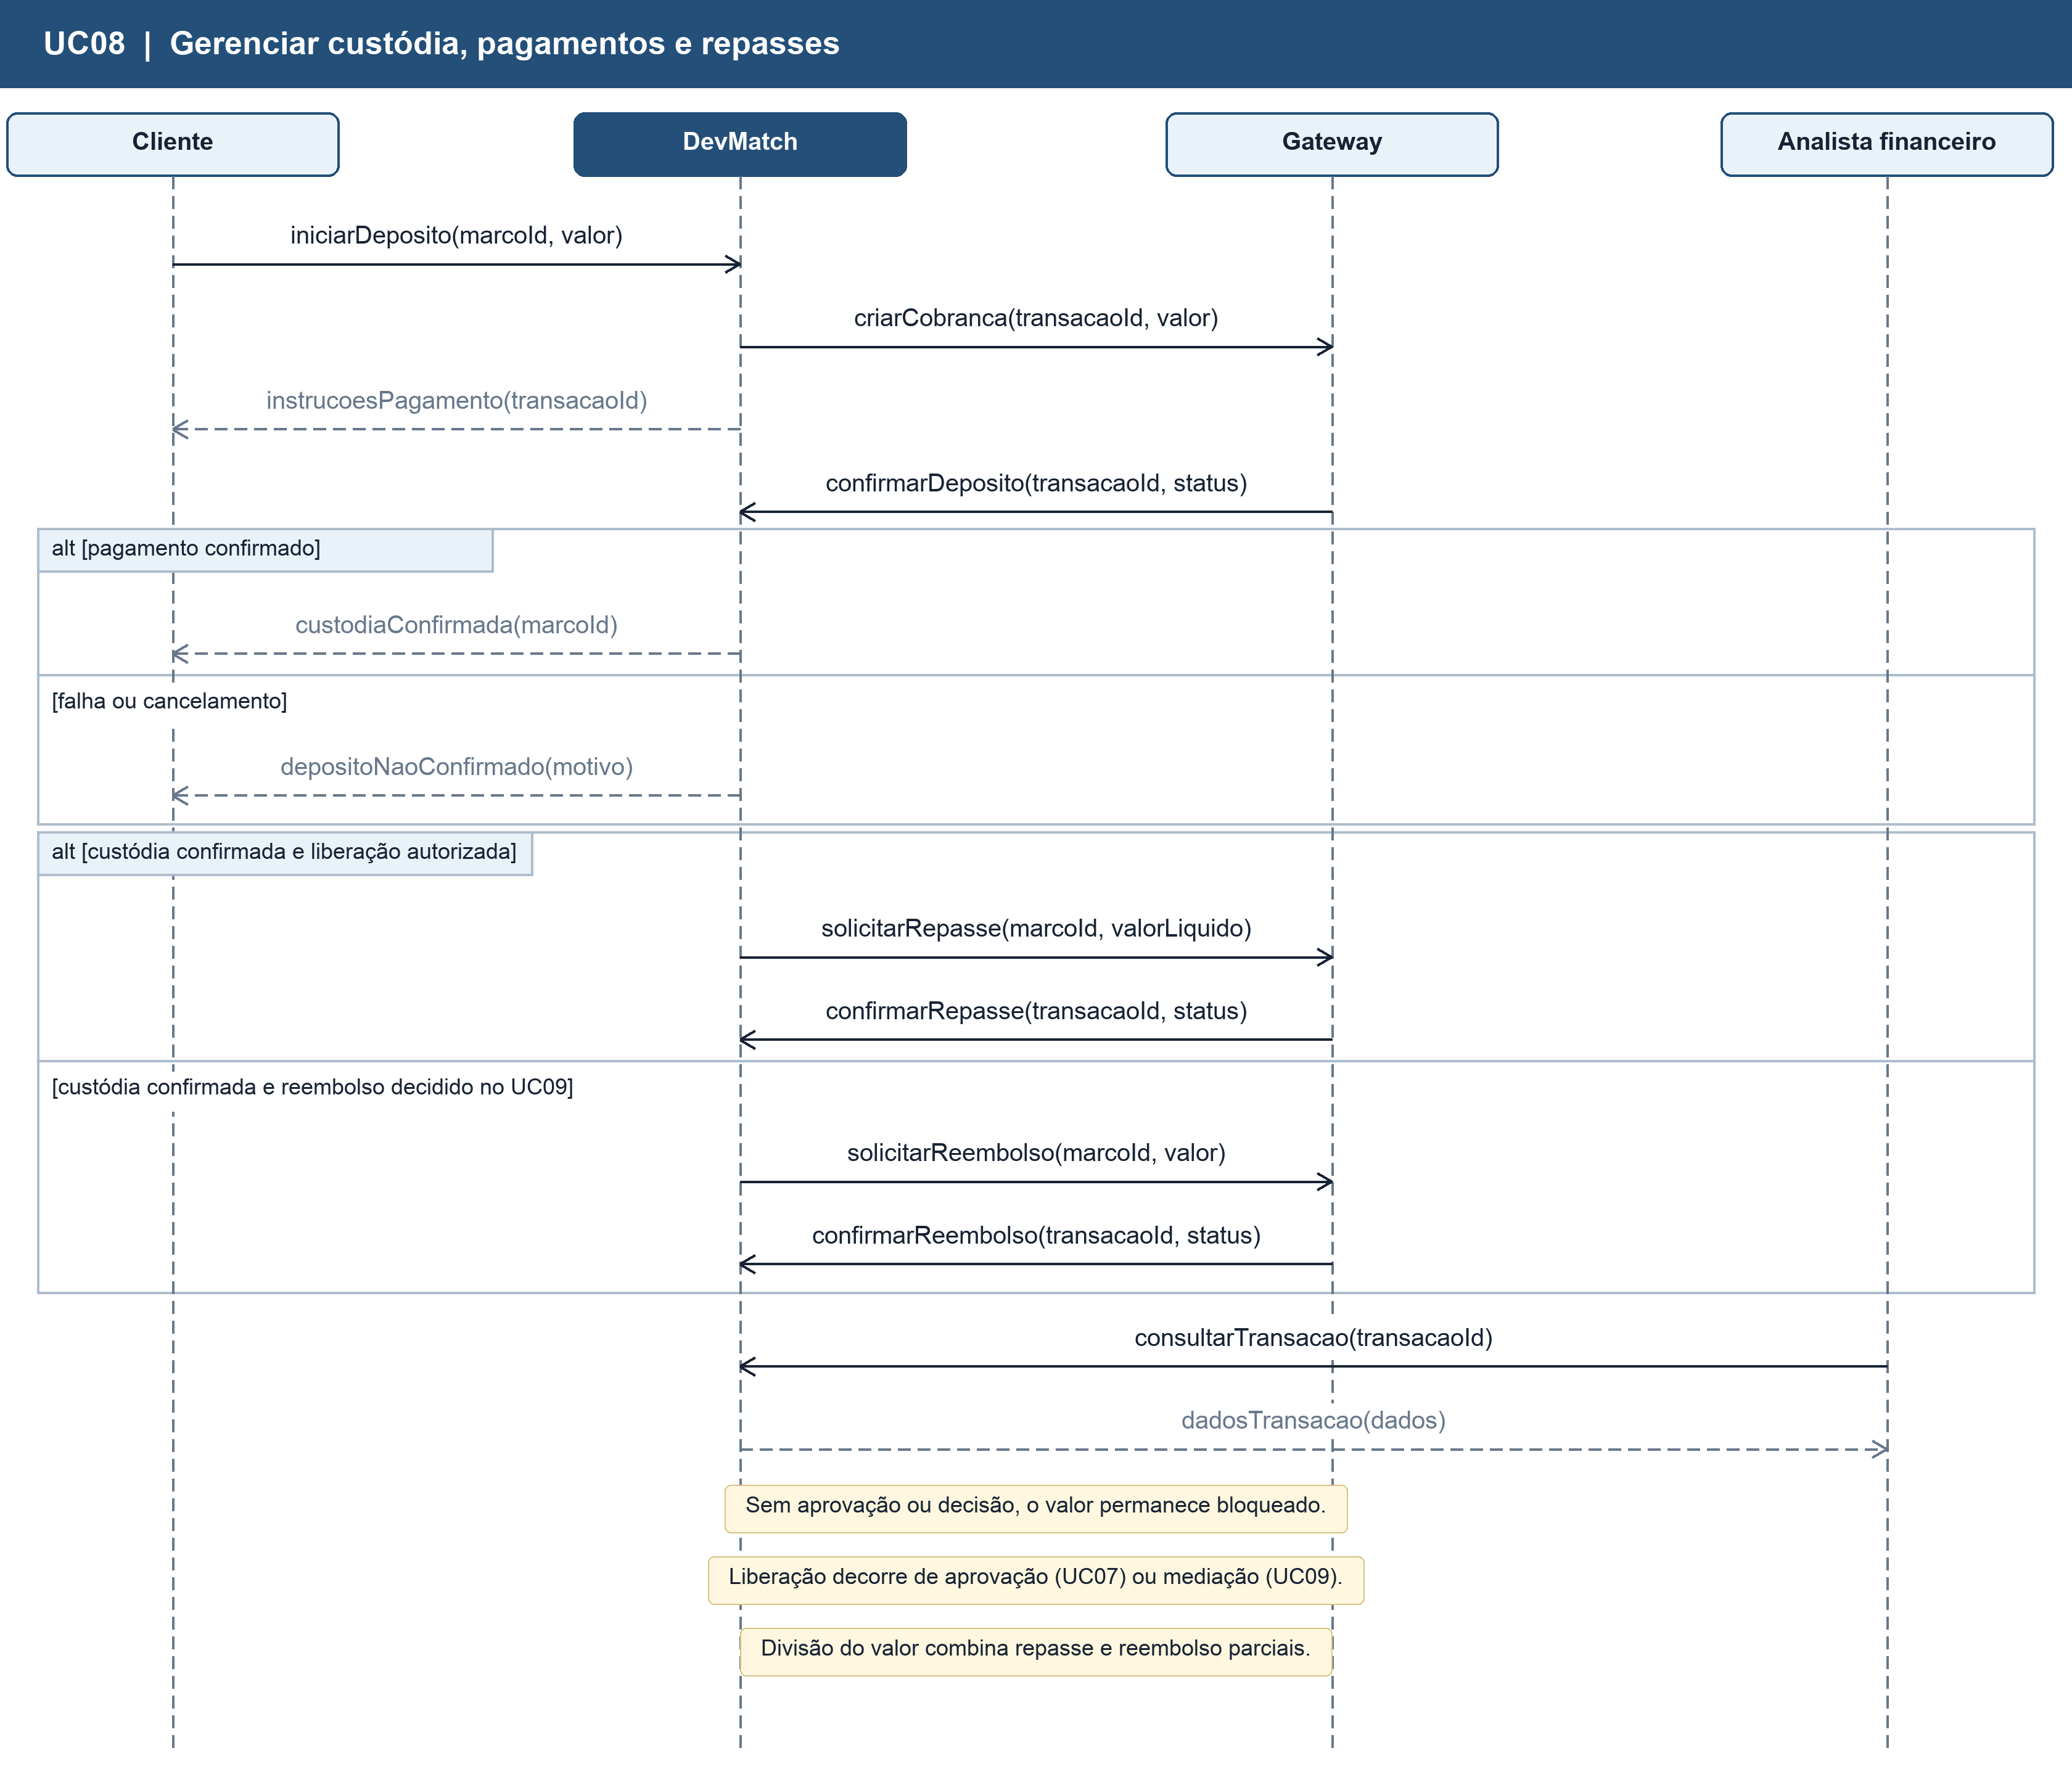
\includegraphics[width=\textwidth,height=0.80\textheight,keepaspectratio]{diagramas/dss_uc08.png}
\caption{DSS do UC08: custódia, pagamentos e repasses.}
\label{fig:dss-uc08}
\end{figure*}

\begin{figure*}[!p]
\centering
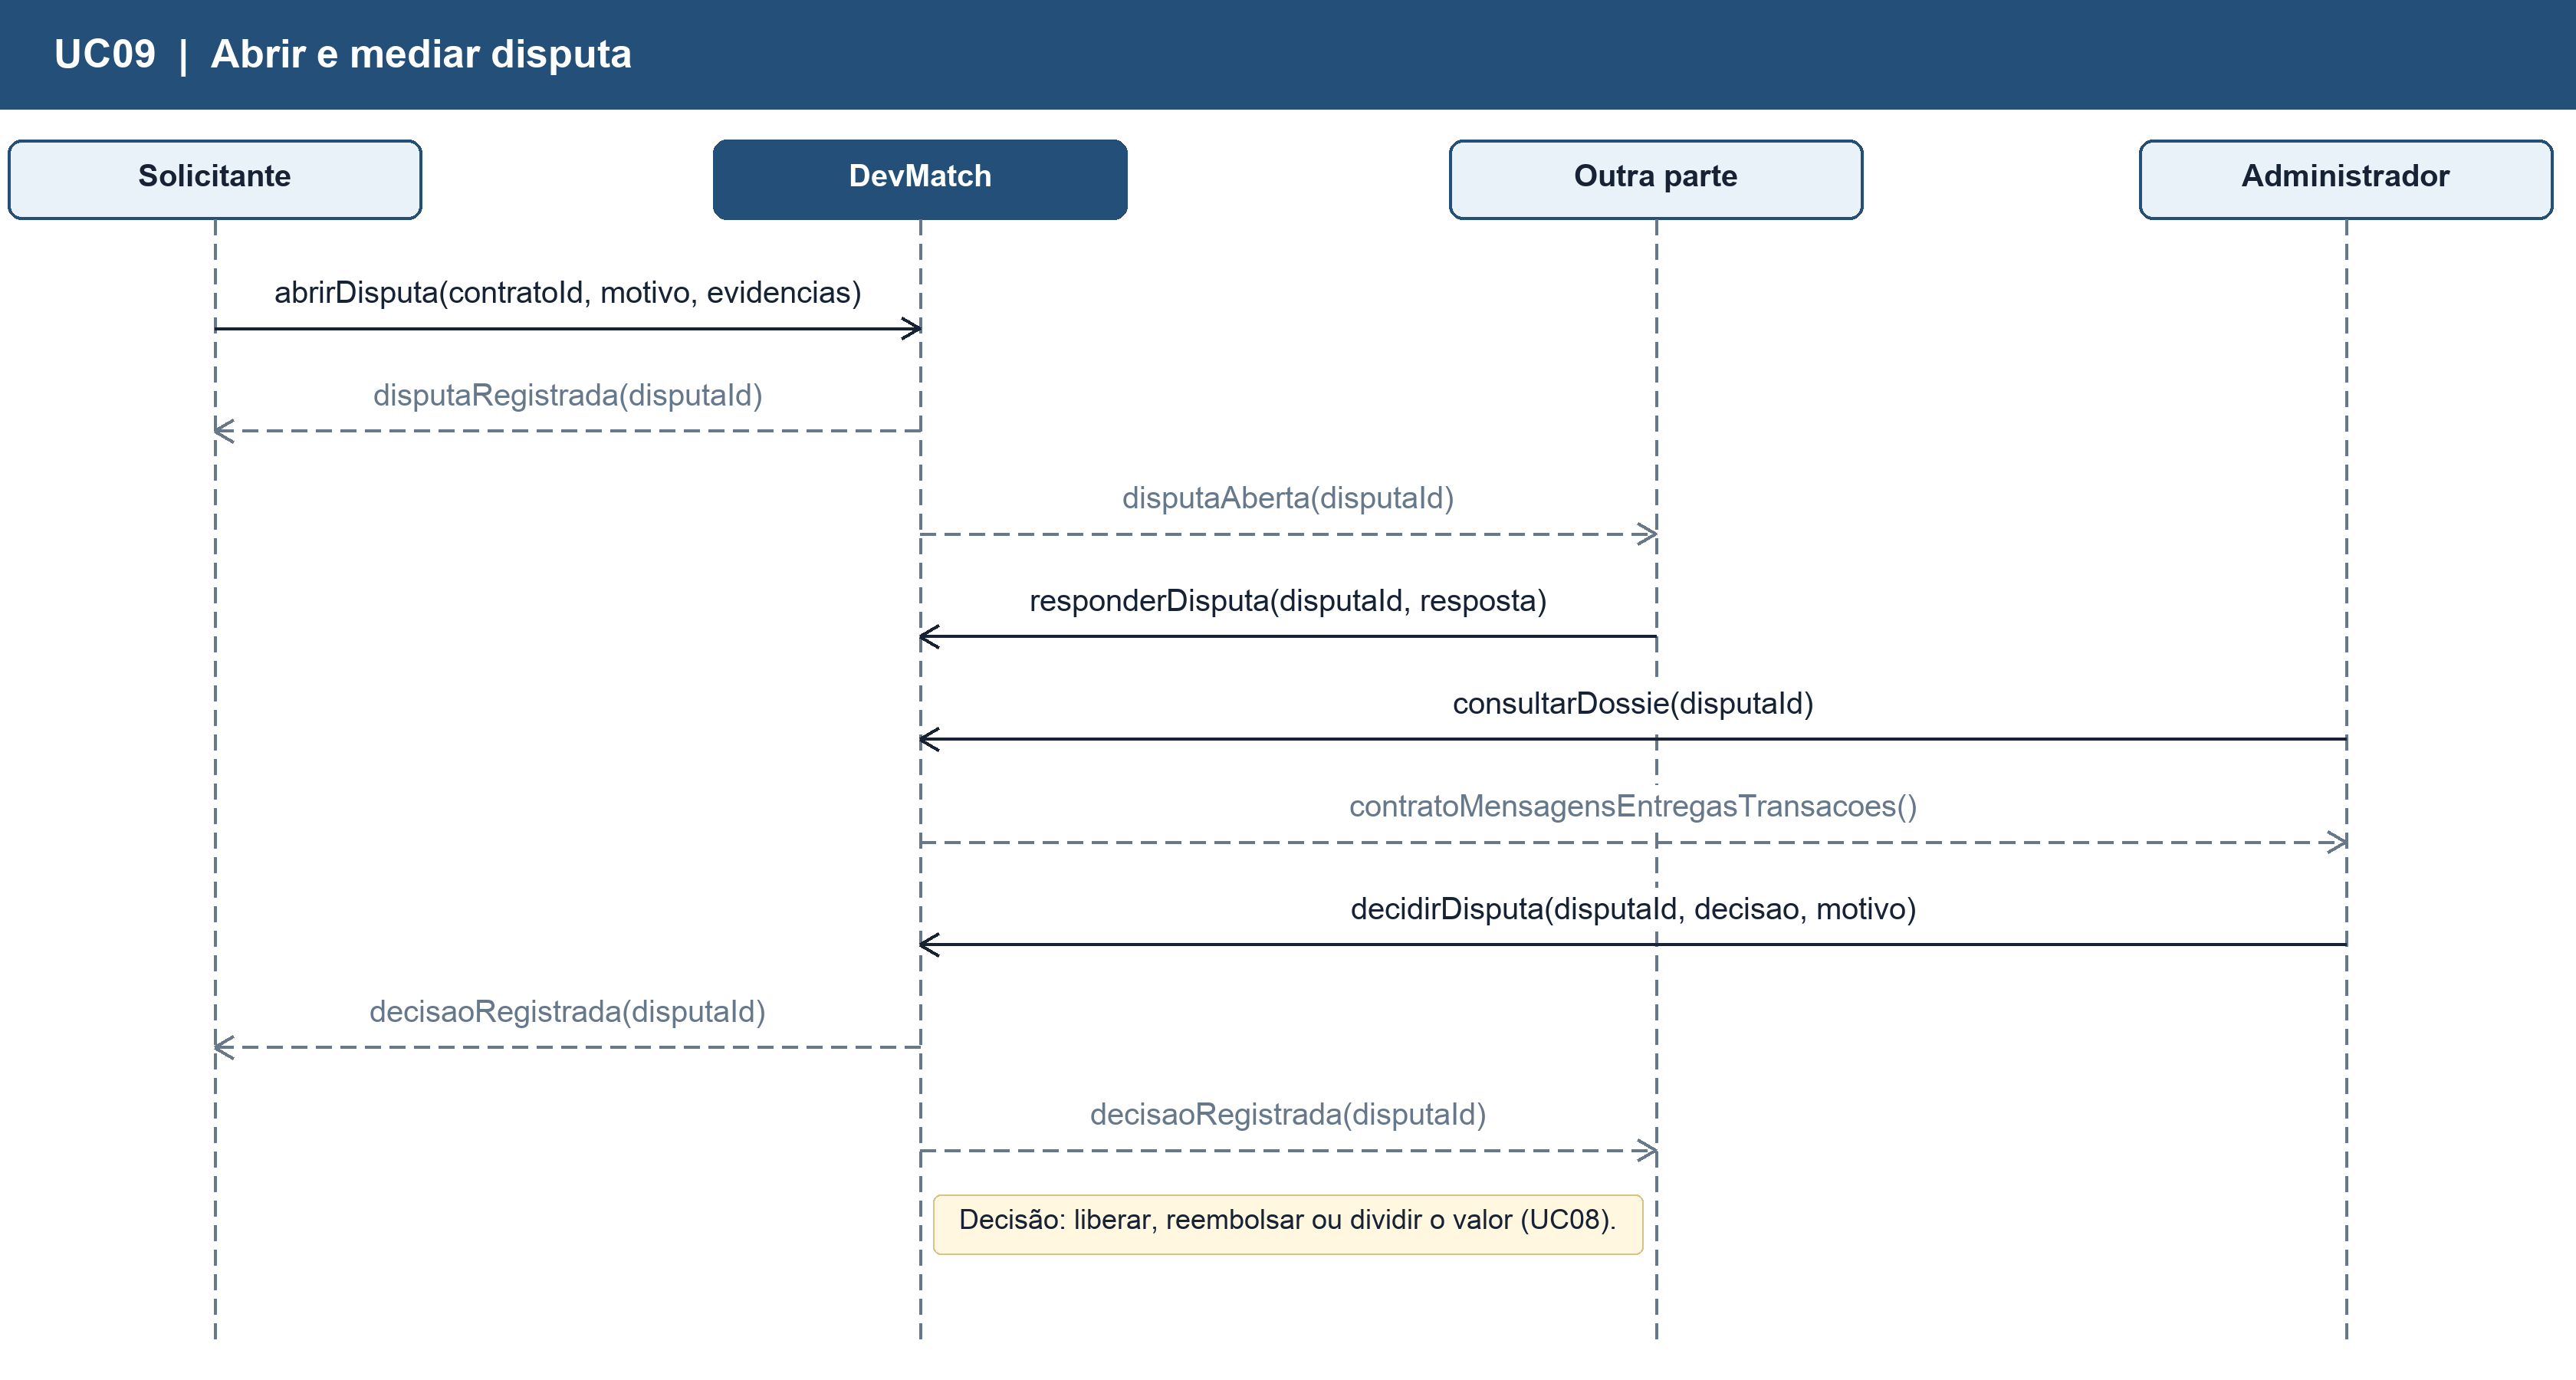
\includegraphics[width=\textwidth,height=0.80\textheight,keepaspectratio]{diagramas/dss_uc09.png}
\caption{DSS do UC09: abertura e mediação de disputa.}
\label{fig:dss-uc09}
\end{figure*}

\clearpage
\subsection{Contratos de Operação dos Casos Centrais}
\label{ap:contratos-operacao}

Os contratos a seguir descrevem o estado necessário antes de cada
operação e os efeitos observáveis depois de sua execução bem-sucedida.
Quando uma pré-condição ou validação não é atendida, o sistema devolve
o motivo da recusa e não produz o efeito de negócio indicado.

\subsubsection{UC03 -- Enviar e negociar proposta}

\paragraph{\texttt{enviarProposta}.}
\textit{Pré-condições:} freelancer autenticado, perfil ativo e projeto
aberto para propostas. \textit{Pós-condições:} uma proposta com valor,
prazo e observações válidos é registrada com identificador e estado
``enviada''; o cliente é notificado.

\paragraph{\texttt{proporAlteracao}.}
\textit{Pré-condições:} solicitante participa da negociação e a
proposta não está encerrada. \textit{Pós-condições:} uma nova versão
dos termos é registrada, o histórico anterior é preservado e a outra
parte é notificada.

\paragraph{\texttt{responderNegociacao}.}
\textit{Pré-condições:} destinatário autorizado e versão pendente de
resposta. \textit{Pós-condições:} a resposta e a situação da
negociação são registradas, com preservação das versões. A seleção
do freelancer para contratação permanece no UC05.

\subsubsection{UC04 -- Publicar e gerenciar projeto}

\paragraph{\texttt{publicarProjeto}.}
\textit{Pré-condições:} cliente autenticado; título, escopo,
orçamento, prazo, tecnologias e critérios de aceitação informados.
\textit{Pós-condições:} o projeto validado recebe identificador,
fica aberto para propostas e se torna pesquisável e elegível para
recomendação.

\paragraph{\texttt{editarProjeto}.}
\textit{Pré-condições:} cliente é responsável pelo projeto e as
alterações não modificam termos de propostas já negociadas.
\textit{Pós-condições:} os dados permitidos são atualizados, com
registro da alteração; propostas anteriores preservam seus termos.

\paragraph{\texttt{pausarProjeto}.}
\textit{Pré-condições:} cliente responsável e projeto aberto.
\textit{Pós-condições:} o projeto passa ao estado ``pausado'' e deixa
de receber novas propostas enquanto a pausa vigorar.

\paragraph{\texttt{encerrarProjeto}.}
\textit{Pré-condições:} cliente responsável e projeto aberto ou
pausado. \textit{Pós-condições:} o projeto passa ao estado
``encerrado'', não recebe novas propostas e preserva contratos e
registros já existentes.

\subsubsection{UC06 -- Formalizar e acompanhar contrato}

\paragraph{\texttt{formalizarContrato}.}
\textit{Pré-condições:} proposta aceita no UC05, cliente autorizado e
marcos compatíveis com o escopo, prazo e valor acordados.
\textit{Pós-condições:} o contrato é criado com escopo, valor, prazo,
responsabilidades e marcos; seu estado fica pendente de confirmação
das partes e de custódia.

\paragraph{\texttt{confirmarContrato}.}
\textit{Pré-condições:} solicitante é uma das partes do contrato e
os termos estão pendentes de sua confirmação. \textit{Pós-condições:}
o aceite é registrado e auditado; o contrato se torna ativo somente
quando as duas partes confirmam e o depósito exigido é validado no
UC08.

\paragraph{\texttt{consultarContrato}.}
\textit{Pré-condições:} solicitante participa do contrato.
\textit{Pós-condições:} o sistema retorna termos, marcos e situação
atual, sem modificar o contrato.

\paragraph{\texttt{proporAlteracaoContrato}.}
\textit{Pré-condições:} contrato ativo e solicitante participante.
\textit{Pós-condições:} a proposta de alteração é registrada e
comunicada à outra parte; os termos vigentes permanecem inalterados
até a confirmação de ambas as partes.

\paragraph{\texttt{confirmarAlteracaoContrato}.}
\textit{Pré-condições:} há alteração pendente e o solicitante é a
outra parte do contrato. \textit{Pós-condições:} os novos termos
passam a vigorar e as versões e confirmações ficam registradas para
auditoria.

\subsubsection{UC07 -- Gerenciar marcos e entregas}

\paragraph{\texttt{registrarEntrega}.}
\textit{Pré-condições:} freelancer participa de contrato ativo e o
marco admite entrega. \textit{Pós-condições:} descrição, data e
artefatos ou links são associados ao marco; a entrega fica pendente
de avaliação e o cliente é notificado.

\paragraph{\texttt{avaliarEntrega}.}
\textit{Pré-condições:} cliente participa do contrato e a entrega
aguarda sua avaliação. \textit{Pós-condições:} a aprovação conclui a
entrega e inicia o repasse no UC08; a solicitação de ajustes exige
justificativa, mantém o pagamento bloqueado e notifica o freelancer.
Se o prazo expirar, aplica-se a regra prevista no contrato.

\subsubsection{UC08 -- Gerenciar custódia, pagamentos e repasses}

\paragraph{\texttt{iniciarDeposito}.}
\textit{Pré-condições:} cliente participa do contrato, o marco exige
provisão e o valor corresponde às condições acordadas.
\textit{Pós-condições:} é criada uma transação com identificador e
estado pendente; o \textit{gateway} recebe a solicitação de cobrança.

\paragraph{\texttt{confirmarDeposito}.}
\textit{Pré-condições:} evento autenticado do \textit{gateway} e
transação existente. \textit{Pós-condições:} se confirmado, o valor
fica bloqueado em custódia e o contrato pode ser ativado após o aceite
das partes; falha ou cancelamento é registrado sem marcar a custódia
como provisionada.

\paragraph{\texttt{confirmarRepasse}.}
\textit{Pré-condições:} evento autenticado do \textit{gateway} e
repasse solicitado após aprovação do marco ou decisão de mediação.
\textit{Pós-condições:} sucesso ou falha é registrado; no sucesso, o
valor líquido e a comissão são conciliados e auditados.

\paragraph{\texttt{confirmarReembolso}.}
\textit{Pré-condições:} evento autenticado do \textit{gateway} e
reembolso autorizado por decisão ou regra contratual.
\textit{Pós-condições:} sucesso ou falha e o valor devolvido são
registrados, conciliados e auditados.

\paragraph{\texttt{consultarTransacao}.}
\textit{Pré-condições:} solicitante possui permissão financeira ou
participa do contrato relacionado. \textit{Pós-condições:} o sistema
retorna tipo, valor e situação da transação, sem alterá-la.

\subsubsection{UC09 -- Abrir e mediar disputa}

\paragraph{\texttt{abrirDisputa}.}
\textit{Pré-condições:} solicitante participa do contrato e informa
justificativa para o desacordo. \textit{Pós-condições:} a disputa e
suas evidências são registradas; o valor relacionado permanece
bloqueado e a outra parte é notificada.

\paragraph{\texttt{responderDisputa}.}
\textit{Pré-condições:} solicitante é a outra parte e a disputa está
aberta. \textit{Pós-condições:} resposta e evidências adicionais são
anexadas ao processo, com preservação do histórico.

\paragraph{\texttt{consultarDossie}.}
\textit{Pré-condições:} administrador autorizado e disputa
registrada. \textit{Pós-condições:} são apresentados contrato,
mensagens, entregas e transações pertinentes; o acesso é auditado
sem alterar o processo.

\paragraph{\texttt{decidirDisputa}.}
\textit{Pré-condições:} administrador autorizado, disputa aberta e
decisão fundamentada nas evidências. \textit{Pós-condições:} decisão e
justificativa são registradas e auditadas; as partes são notificadas
e a liberação, devolução ou divisão do valor é encaminhada ao UC08.


% ============================================================
% DECLARAÇÕES
% ============================================================

\begin{declarations}

\begin{contributions}
Antônio Henrique Rabelo Andrade contribuiu para o levantamento e a
modelagem dos requisitos, a descrição dos atores, a elaboração dos
casos de uso e histórias de usuário e a redação da introdução,
resumo e abstract.

% Acrescentar aqui as contribuições dos demais integrantes.

Todos os autores leram e aprovaram a versão final do manuscrito.
\end{contributions}

\begin{interests}
Os autores declaram que não têm nenhum conflito de interesses.
\end{interests}

\begin{materials}
Os modelos, diagramas e demais materiais produzidos neste trabalho
serão disponibilizados mediante solicitação.
\end{materials}

\begin{aitools}
Foi utilizada uma ferramenta de inteligência artificial generativa,
ChatGPT, para auxiliar na organização textual, revisão linguística
e formatação inicial de trechos em LaTeX. Os autores revisaram e
validaram o conteúdo produzido e permanecem responsáveis por todas
as informações apresentadas no trabalho.
\end{aitools}

\begin{furtherinformation}
Este trabalho possui finalidade acadêmica e concentra-se na
especificação e modelagem de um sistema de software. Não foram
realizadas pesquisas ou experimentos envolvendo seres humanos.
\end{furtherinformation}

\end{declarations}

% ============================================================
% REFERÊNCIAS
% ============================================================

\bibliographystyle{apalike-sol}
\bibliography{refs}

\end{document}
